%\documentclass[11pt]{report}
%\usepackage{siunitx}
%\usepackage{graphicx}
%\usepackage{makecell}
%\usepackage{booktabs}
%\usepackage[table,xcdraw]{xcolor}
%
%\begin{document}
%\setcounter{chapter}{5}
%\tableofcontents


\newpage
\chapter{Development of a novel bioreactor methodology: \textit{JANUS}}
This chapter explains the development of a novel bioreactor under an introduced methodology driven by numerical predictions. The resultant bioreactor was codenamed JANUS, which refers to the Roman god that represented a duality, here meaning a simultaneous physical and digital entity. The developed concept allows it to be easily fabricated with low-cost 3D printing, while simultaneously allowing the construction of precise microenvironment numerical models, unlocking predictions of important cell culture parameters for enhanced control and actuation. The created bioreactor concept is open source, highly replicable, and available to other research groups. This chapter traces the history behind this development. Its contents were collected from the following works:
\begin{itemize}
\item \small \textit{João Meneses, João C Silva, Sofia R Fernandes, Abhishek Datta, Frederico Castelo Ferreira, Carla Moura, Sandra Amado, Nuno Alves, and Paula Pascoal-Faria. 2020. “A Multimodal Stimulation Cell Culture Bioreactor for Tissue Engineering: A Numerical Modelling Approach.” Polymers 12 (4).};
\item \small \textit{João Meneses, Sofia R Fernandes, João C Silva, Frederico Castelo Ferreira, Nuno Alves and Paula Pascoal-Faria. 2023. ''JANUS: an open-source 3D printable perfusion bioreactor and numerical model-based design strategy for tissue engineering''. Front. Bioeng. Biotechnol. 11:1308096.};
\end{itemize}
This chapter's required cell culture procedures were made in collaboration with the SCERG - Stem Cell Engineering Research Group from iBB/IST - Instituto Superior Técnico, Portugal.
\newpage 




\section{Introduction}
Bioreactors for \textit{in vitro} cultures are increasingly used in \acs{TE} due to more complex mass transport requirements of growing tissues, and also to allow controlled reproduction of specific cellular environments that can promote particular cellular processes by applying stimulation (e.g., mechanical, electrical). Understanding the microenvironment generated by bioreactors is crucial to predict cell survival and fate in TE strategies \cite{Reina-Romo2019-ry}. \textit{In silico} models have been successfully applied to guide the development and optimization steps towards a bioreactor design that favors the best cellular outcomes regarding seeding, proliferation, and differentiation \cite{Engel2021-fk, Spencer2013-pg, Perier-Metz2021-bj}. Growing evidence reports multiple important environmental properties, like dissolved oxygen tension, glucose and lactate concentrations, and local pH value, that can strongly impact stem cell fate. They should be closely monitored and controlled \cite{Klein2021-dz, Klein2022-yj, Monfoulet2014-ef, Seddiqi2020-uo, Beskardes2018-fq}, regardless of how difficult and time/resource consuming can be to monitor and control specific cell microenvironments simultaneously. Predictions from computational studies help to determine the most relevant factors in the evolution and dynamics of biological systems \cite{Geris2018-tz}, optimizing control and modulation of cell cultures in bioreactor systems in a low-cost virtual environment.

Many bioreactor designs have been proposed in \acs{TE} to support better the proliferation and differentiation of several cell populations \cite{Smith2018-he, Montorsi2022-qm}. Some bioreactors include a specific set of sensors to allow improved monitorization of the \textit{in vitro} environmental conditions or actuator systems to apply different types of physical stimuli to promote cell differentiation (e.g., electric field, magnetic field, mechanical stress) \cite{Lim2022-dr}. Even if proven effective, most of these designs are not shared open-source with proper fabrication and integration instructions, which hinders reproducibility and usage by the \acs{TE} research community. The global massification of \acs{3D} printing technologies unlocks the opportunity to construct complex perfusion structures in suitable materials and techniques, while retaining high customization freedom, reproducibility, and shareability at a low cost \cite{Gensler2020-in, Haleem2020-oj}.

The considered workflow for developing a bioreactor consists of a series of interchained steps, as shown in Figure \ref{figWorkflow}. The first considered stage focused on the pre-design validation of construction materials and methods (spanning \acs{3D} printing technologies), including, if required, any material post-processing after fabrication. This stage of work was published in MDPI Polymers Journal under the title: "A Multimodal Stimulation Cell Culture Bioreactor for Tissue Engineering: A Numerical Modelling Approach" \cite{Meneses2020-dx}, presenting one of the first attempts to create a multimodal (mechanical and electric stimulation) perfusion bioreactor design along with its numerical models.

\begin{figure}
\makebox[\textwidth][c]{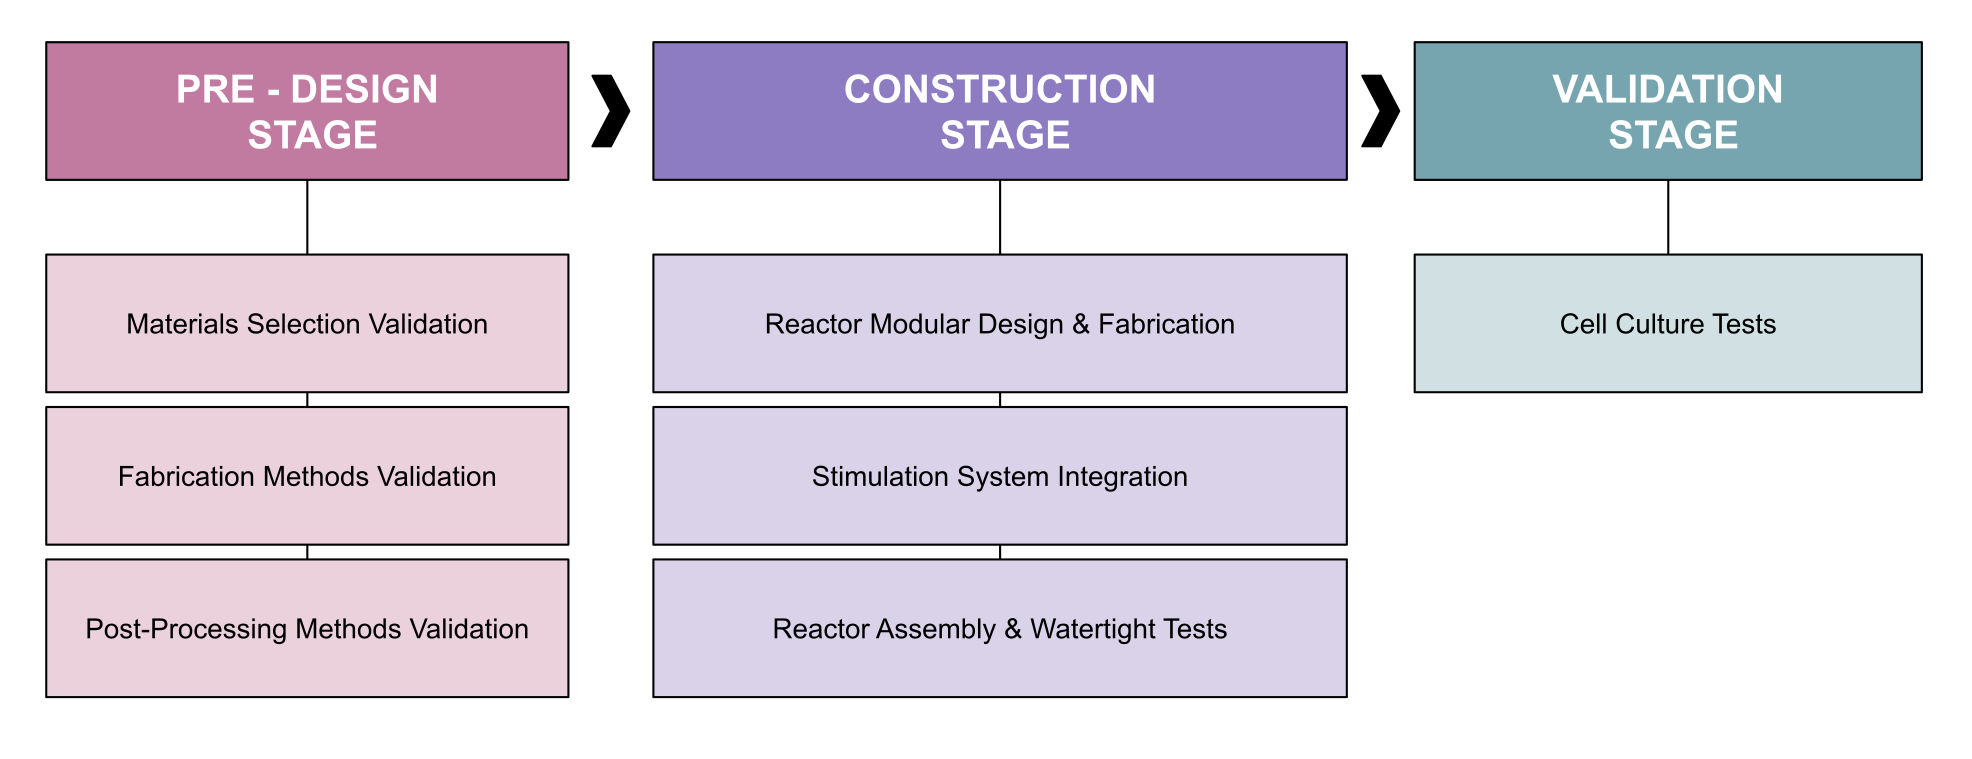
\includegraphics[scale=0.6]{figures/Figure_6d1}}
\caption{Workflow steps planned for the \textit{JANUS} bioreactor development, grouped by stages.}
\label{figWorkflow}
\end{figure}   

Recently we published the progress made in the construction and validation stages. A strategy was envisioned to iteratively design a perfusion bioreactor system based on model-driven decisions made on the microenvironment generated by each design hypothesis.  These decisions aim to obtain cell culture conditions that promote a particular cell line's high proliferation and differentiation rates (e.g., mesenchymal stem/stromal cells \cite{Bianconi2023-rs, Alvarez-Barreto2011-lj}, embryonic stem cells \cite{Marolt2012-xc}, induced pluripotent stem cells \cite{De_Peppo2013-dq}). Perfusion technology was selected due to its natural double role in bioreactor systems allowing the renovation of the culture medium and, at the same time, applying fluid flow-induced wall shear stress stimuli to the tissue constructs, which has been shown to enhance MSC-mediated bone formation \textit{in vitro} \cite{Wittkowske2016-xr, Schroder2022-qt, Yamada2022-aq}. For each microenvironment, \acs{FEM} models were used to predict the volumetric distributions of fluid flow-induced shear stress and \acs{EF} magnitude in culture regions. The proposed perfusion bioreactor system can be fabricated with \acs{3D} printing technologies (e.g., fused filament fabrication, stereolithography) and accommodates the capability for simultaneous electrical and mechanical stimulation of four scaffolds in identical conditions. The journey pursued to get the proposed bioreactor design is presented, from early conceptualization to the current version, following a multiple trial and error approach. The strategy of early integrating numerical models of the bioreactor-generated microenvironment into the design phase allows trying different stimulation protocols and geometric options before fabrication, saving time and reducing operational costs. After fabrication, we experimentally validated the bioreactor system outputs against their numerical model outputs to increase the confidence in the developed strategy, obtaining a digital twin of the experimental setup capable of improving environmental control of cell cultures and, at the same time, capable of providing a framework to study the cellular effects of the applied stimuli. The complete developed solution, including all bioreactors' components and numerical models, was named JANUS. This Roman inspiration describes here a duality of physical and virtual representations. JANUS is available in an online repository (https://doi.org/10.5281/zenodo.7695700, released under an open-source Attribution-ShareAlike 4.0 International license). JANUS approach can be potentially applied to any cell culture study in the context of \acs{TE} without any loss of applicability. Nevertheless, to establish design goals and allow \textit{in vitro} validation, we directed the current development to \acs{BTE} using a specific bone cell line since it constitutes an active research topic and a necessity to progress the understanding in this TE field of research \cite{Sladkova2014-yw}. The presented bioreactor development was motivated by successive approaches to deliver adequate in vitro mechanical and electrical stimulation conditions to bone cells seeded on 3D-printed porous PCL scaffolds, in order to generate an osteogenic stimulation protocol that may mimic the native human bone microenvironment, and consequently, improve the regenerative outcomes.

\begin{figure}
\makebox[\textwidth][c]{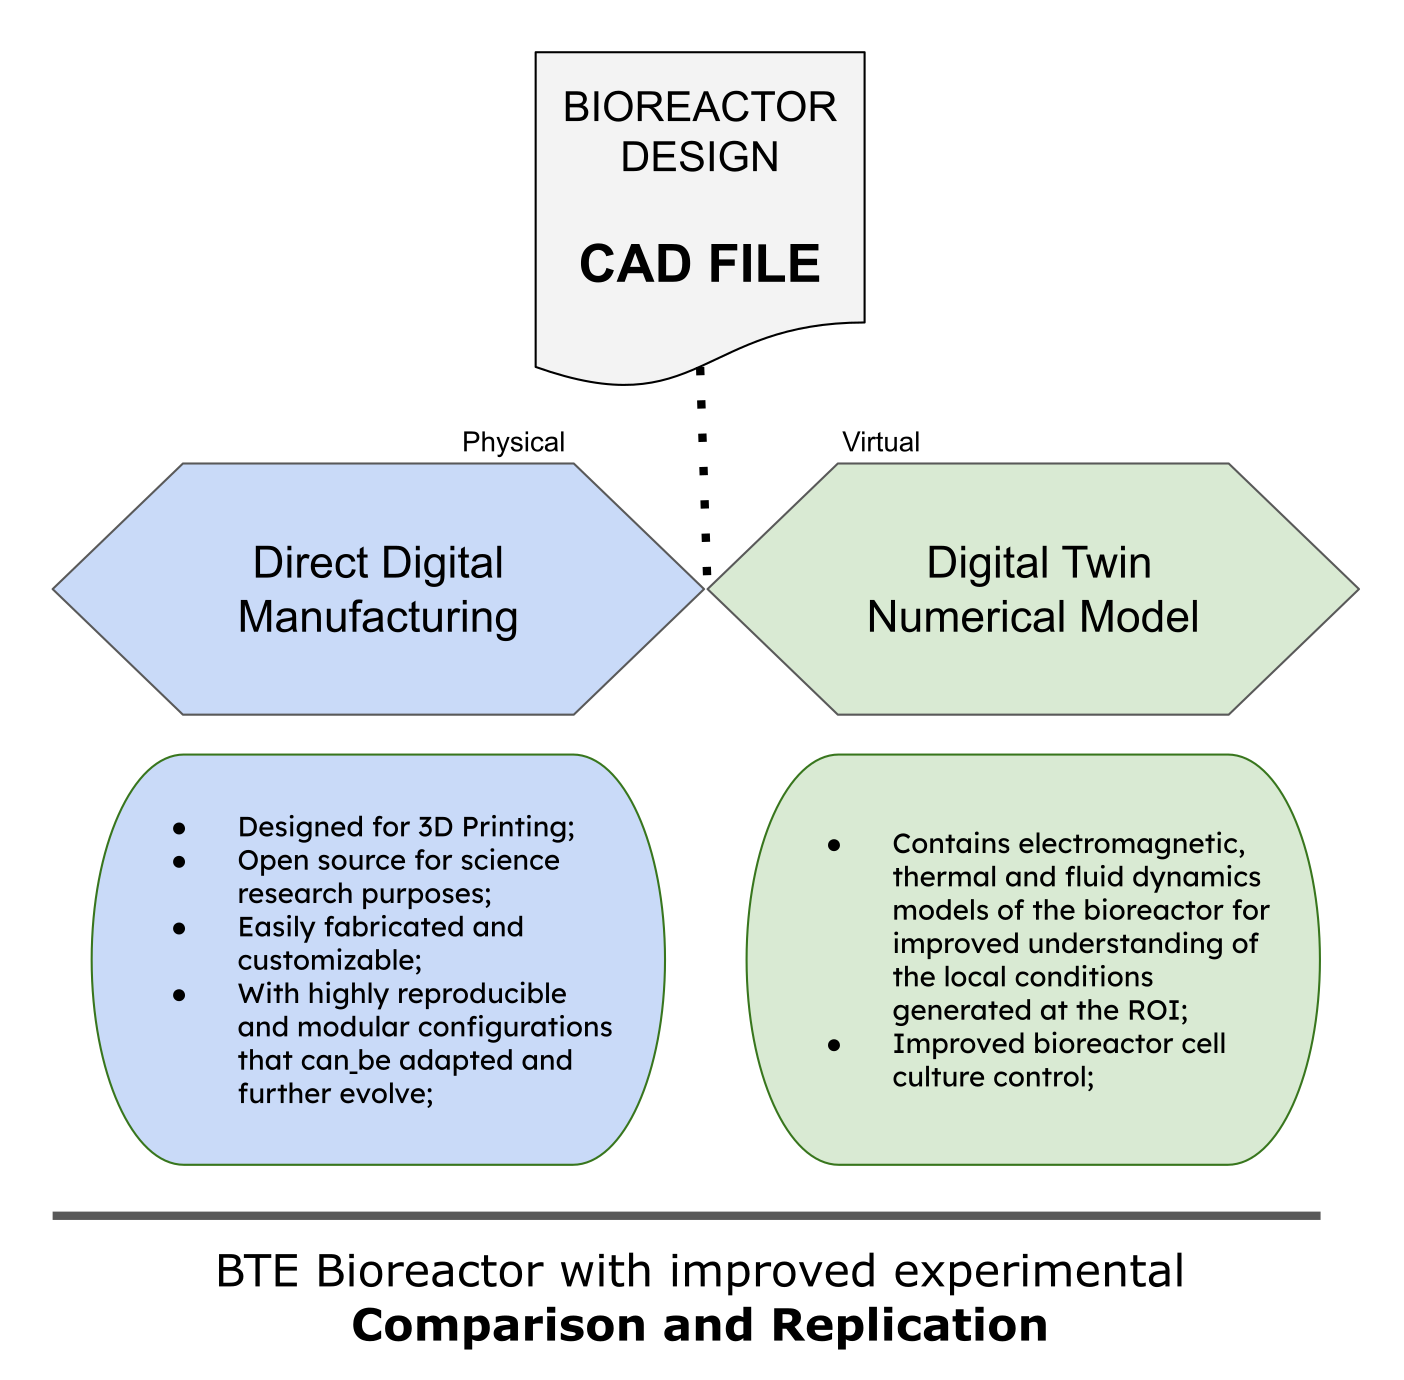
\includegraphics[scale=0.6]{./figures/Figure_6d2}}
\caption{The JANUS bioreactor duality concept based in a shared root \acs{CAD} file, using this standard file to create detailed methodologies for physical and virtual replication.}
\label{figCadFile}
\end{figure}  

The proposed JANUS bioreactor duality (physical and virtual entity) concept is built on top of a geometrical design \acs{CAD} file, see Figure \ref{figCadFile}. With this file, all structures, components, and parts of the bioreactor (including any existing scaffold structure) could be geometrically represented with accurate dimensions and in their experimental position. The \acs{CAD} file can easily be shared among scientists to be used in two ways: first, to replicate the bioreactor concept through additive and/or subtractive construction methods (assuming that all construction methodologies are also shared with sufficient detail); second, to run bioreactor numerical models based on \acs{FEM} analysis, allowing to predict, test and optimize physical/chemical microenvironments. This combination of capabilities allows for continuously improved bioreactor design and control of generated environments, impacting experimental replicability.




\section{Aim}
\begin{itemize}
\item Validate an adequate biocompatible material after being produced by additive manufacturing method and post-processed to fabricate a bioreactor part; 
\item Design a multimodal stimulation perfusion bioreactor based on numerically model-driven decisions made on the microenvironment generated by each design hypothesis;
\item With the designed bioreactor \acs{CAD} file, fabricate the physical bioreactor with \acs{3D} printing technologies and simultaneously create the bioreactor digital model;
\item Validate the fabricated bioreactor design, confirming its stimulation outputs against their corresponding numerical models. Run preliminary \textit{in vitro} cell culture tests.
\end{itemize}




\section{Methods}


\subsection{Material samples production}
This process goal was to simultaneously validate an adequate biocompatible material, additive manufacturing method, and post-processing steps to fabricate a bioreactor. To do so, simple parallelepiped samples with dimensions of 10 \si{\milli\meter} of depth, 10 \si{\milli\meter} of width and 5 \si{\milli\meter} of height were drawn in SOLIDWORKS 2018 Student Edition (Dassault Sistèmes), and then exported to the stereolithography file format (*.stl). This file was then imported to each additive manufacturing technology native software as described in Table \ref{tabMat}. All samples from the same material were printed under the same conditions. Table \ref{tabMat} summarises the type and additive manufacturing methodology for each material sample fabricated. Materials used were selected based on additive manufacturing compatibility, suitable mechanical properties, cost, easy processing, and material transparency. The latter feature may play a key role in real-time visualization of the scaffold during \textit{in vitro} bioreactor cultures.   
 
\begin{table}
\caption{Description of tested samples identity (ID), material, correspondent supplier, and additive manufacturing methodology.}
\bigskip
\tiny
\centering
\begin{tabularx}{325px}{c c l l} \toprule[0.15em]
\textbf{Sample ID}	& \textbf{Material}	& \textbf{Supplier} & \textbf{AM Methodology}\\ \cmidrule(l){1-4}

PCL & Polycaprolactone 
& \makecell[l]{FACILAN™ PCL 100,\\ 750 GRAM (MW: 50000 g/mol),\\ 1.75 MM,\\ 3D4MAKERS,\\ Haarlem, The Netherlands}
& \makecell[l]{
3DP Technology: FDM;\\
3D Printer: Creatbot F430;\\
Nozzle Diameter: 0.4 \si{\milli\meter};\\
Nozzle Temperature: 165 \si{\celsius};\\
Heated Bed Temperature: 35 \si{\celsius};\\
Chamber Temperature: 20 \si{\celsius};\\
Printing Speed: 60 \si{\milli\meter\per\second};\\
Infil: 100 \si{\percent}.}
\\ \cmidrule(l){1-4}
PA			
& Polyamide/Nylon			
& \makecell*[l]{PA Powder,\\ 3D SYSTEMS}		
& \makecell*[l]{3DP Technology: SLS;\\
3D Printer: 3D System sPro 60 HD-HS;\\
CO2 Laser 70 \si{\watt};\\
Layer Thickness:  0.1 \si{\milli\meter};\\
Scanning Speed: 6 \si{\meter\per\second};\\
Construction Chamber Temperature: 173 \si{\celsius};\\
Feeding Chamber Temperature: 135 \si{\celsius}.}
\\ \cmidrule(l){1-4}
PETG			
& \makecell{Polyethylene\\ Terephthalate\\ Glycol-modified}
& \makecell[l]{PETG FILAMENT,\\ 750 GRAM,\\ 1.75MM,\\ 3D4MAKERS,\\ Haarlem, The Netherlands}
& \makecell[l]{
3DP Technology: FDM;\\
3D Printer: Creatbot F430;\\
Nozzle Diameter: 0.4 \si{\milli\meter};\\
Nozzle Temperature: 260 \si{\celsius};\\
Heated Bed Temperature: 110 \si{\celsius};\\
Chamber Temperature: 60 \si{\celsius};\\
Printing Speed: 60 \si{\milli\meter\per\second};\\
Infil: 100 \si{\percent}.}
\\ \cmidrule(l){1-4}
ABS		
& \makecell{Acrylonitrile-\\Butadiene-\\Styrene}
& \makecell[l]{ABS FILAMENT,\\ 750 GRAM,\\ 1.75MM,\\ 3D4MAKERS, Haarlem,\\ The Netherlands}
& \makecell[l]{
3DP Technology: FDM;\\
3D Printer: Creatbot F430;\\
Nozzle Diameter: 0.4 \si{\milli\meter};\\
Nozzle Temperature: 230 \si{\celsius};\\
Heated Bed Temperature: 50 \si{\celsius};\\
Chamber Temperature: 35 \si{\celsius};\\
Printing Speed: 60 \si{\milli\meter\per\second};\\
Infil: 100 \si{\percent}.}
\\ \cmidrule(l){1-4}
C8		
& \makecell{Proprietary Polymer\\ Composite produced\\ by ELOGIOAM 3D\\ MATERIALS}
& \makecell[l]{FACILAN™ C8 FILAMENT,\\ 750 GRAM,\\ 1.75MM,\\ 3D4MAKERS, Haarlem,\\ The Netherlands}
& \makecell[l]{
3DP Technology: FDM;\\
3D Printer: Creatbot F430;\\
Nozzle Diameter: 0.4 \si{\milli\meter};\\
Nozzle Temperature: 195 \si{\celsius};\\
Heated Bed Temperature: 35 \si{\celsius};\\
Chamber Temperature: 20 \si{\celsius};\\
Printing Speed: 60 \si{\milli\meter\per\second};\\
Infil: 100 \si{\percent}.}
\\ \cmidrule(l){1-4}
PPSU		
& \makecell{Polyphenylsulfone}
& \makecell[l]{PPSU FILAMENT,\\ 500 GRAM,\\ 1.75 MM,\\ 3D4MAKERS, Haarlem,\\ The Netherlands}
& \makecell[l]{
3DP Technology: FDM;\\
3D Printer: Creatbot F430;\\
Nozzle Diameter: 0.4 \si{\milli\meter};\\
Nozzle Temperature: 380 \si{\celsius};\\
Heated Bed Temperature: 120 \si{\celsius};\\
Chamber Temperature: 60 \si{\celsius};\\
Printing Speed: 60 \si{\milli\meter\per\second};\\
Infil: 100 \si{\percent}.}
\\ \cmidrule(l){1-4}
PEEK		
& \makecell{Polyether\\ Ether\\ Ketone}
& \makecell[l]{PEEK FILAMENT,\\ 500 GRAM,\\ 1.75 MM,\\ 3D4MAKERS, Haarlem,\\ The Netherlands}
& \makecell[l]{
3DP Technology: FDM;\\
3D Printer: Creatbot F430;\\
Nozzle Diameter: 0.4 \si{\milli\meter};\\
Nozzle Temperature: 390 \si{\celsius};\\
Heated Bed Temperature: 120 \si{\celsius};\\
Chamber Temperature: 60 \si{\celsius};\\
Printing Speed: 60 \si{\milli\meter\per\second};\\
Infill: 100 \si{\percent}.}
\\ \bottomrule[0.15em]
\end{tabularx}
\label{tabMat}
\end{table}


\subsection{\textit{In vitro} cytotoxicity tests}
The biocompatibility of the different materials considered for the bioreactor fabrication was assessed using L929 mouse fibroblasts (ATCC number CCL-1) and following the ISO 10993-5 and ISO 10993-12 guidelines \cite{For_Standardization2009-wo}. Before the test, the materials were sterilized by ultraviolet exposure overnight, ethanol 70\si{\percent} washing and incubation with a 1\si{\percent} antibiotic--antimycotic (Anti--Anti, Gibco\texttrademark, Fisher Scientific, USA) solution in phosphate-buffered saline (PBS, Gibco\texttrademark, Fisher Scientific, USA). All materials were evaluated by performing the indirect extract test and direct contact test. L929 fibroblasts were cultured on tissue culture polystyrene plates with Dulbecco’s Modified Eagle’s Medium (DMEM, Gibco\texttrademark, Fisher Scientific, USA) supplemented with 10\si{\percent} (\emph{v}/\emph{v}) Fetal Bovine Serum (FBS, LifeTechnologies, USA) and with 1 \si{\percent} Anti--Anti in an incubator at 37 \si{\celsius}/5 \si{\percent} CO$_{2}$, to be used as a negative control. Latex was used as a positive control for cell death. Extracts were prepared by incubating the materials in DMEM + 10 \si{\percent} FBS + 1 \si{\percent} Anti--Anti culture media at a ratio of 0.2 \si{\gram} of material/\si{\milli\liter} for 72 \si{\hour} at 37 \si{\celsius}/ 5 \si{\percent} CO$_{2}$. This ratio ensures that the test sample covers one-tenth of the cell layer surface, according to the ISO 10993-5:2009 \cite{For_Standardization2009-wo}. L929 fibroblasts were seeded on tissue culture polystyrene plates at a cell density of 10$^{5}$ cells per well and cultured for 24 \si{\hour} at 37\si{\celsius}/ 5\si{\percent} CO$_{2}$ to generate a confluent monolayer. For the indirect extract test, the culture media was removed, and L929 cells were exposed to the material extract’s conditioned medium for 72 \si{\hour} at 37\si{\celsius}/ 5\si{\percent} CO$_{2}$. Then, extract conditioned media were removed, and the MTT (3-(4,5-dimethylthiazol-2-yl)-2-5 diphenyl tetrazolium bromide) assay (In Vitro Toxicology Assay Kit MTT based, Sigma-Aldrich, USA) was performed by the manufacturer’s guidelines. Briefly, cells were incubated with MTT solution (1 mg/mL, yellow) for 2\si{\hour} at 37\si{\celsius}. Afterward, the violet formazan product resultant from the MTT metabolic reduction by metabolically active cells was dissolved under agitation using a 0.1 \si{\molar} HCl solution in anhydrous isopropanol (Sigma-Aldrich). Absorbance values of the resultant solutions were measured in a plate reader (Infinite M200 PRO, TECAN, Mannedorf, Switzerland) at 570 \si{\nano\meter}. The direct contact assay was performed by the ISO standards mentioned above. Individual specimens of the test samples were carefully placed over previously formed confluent monolayer of L929 fibroblasts (in the center of each of the replicate wells; three replicates were used for each sample). The materials were in direct contact with the L929 cell monolayer, incubated for 72\si{\hour} at 37\si{\celsius}/ 5\si{\percent} CO$_{2}$, according to the ISO 10993-5:2009 standard. Afterward, cell viability and morphology were evaluated qualitatively under an inverted optical microscope (LEICA DMI3000B, Leica Microsystems, Wetzlar, Germany) equipped with a digital camera (Nikon DXM1200F, Nikon Instruments Inc., Melville, USA) to assess any cytotoxic responses such as the occurrence of halo inhibition effect or abnormal cell morphology.


\subsection{Bioreactor design based on model-driven decisions}
A bottom-top approach to bioreactor design was guided by \acs{FEM} based models. The decision tree applied for the bioreactor development is described in this section in a step-by-step manner (Figure \ref{figStrategy}). A cyclic iteration between \acs{CAD} design and \acs{FEM} predictions is conducted until the established microenvironment for that particular design is achieved. With this approach, we aim to reach a design that, once fabricated, can operate as numerically predicted. We only report here the fundamentals of every development step. A full description is reported in the original manuscript that originated this chapter, along with the complete roadmap of this bioreactor development. A glimpse of the evolution of this bioreactor design concept, main features, and subsequent methodology, defined in this thesis work, can be observed in Figure \ref{figStory}. To facilitate reproducibility, all systems developed in this work have only considered commercially available components or custom-made \acs{3D} printing parts.  

\begin{figure}
\makebox[\textwidth][c]{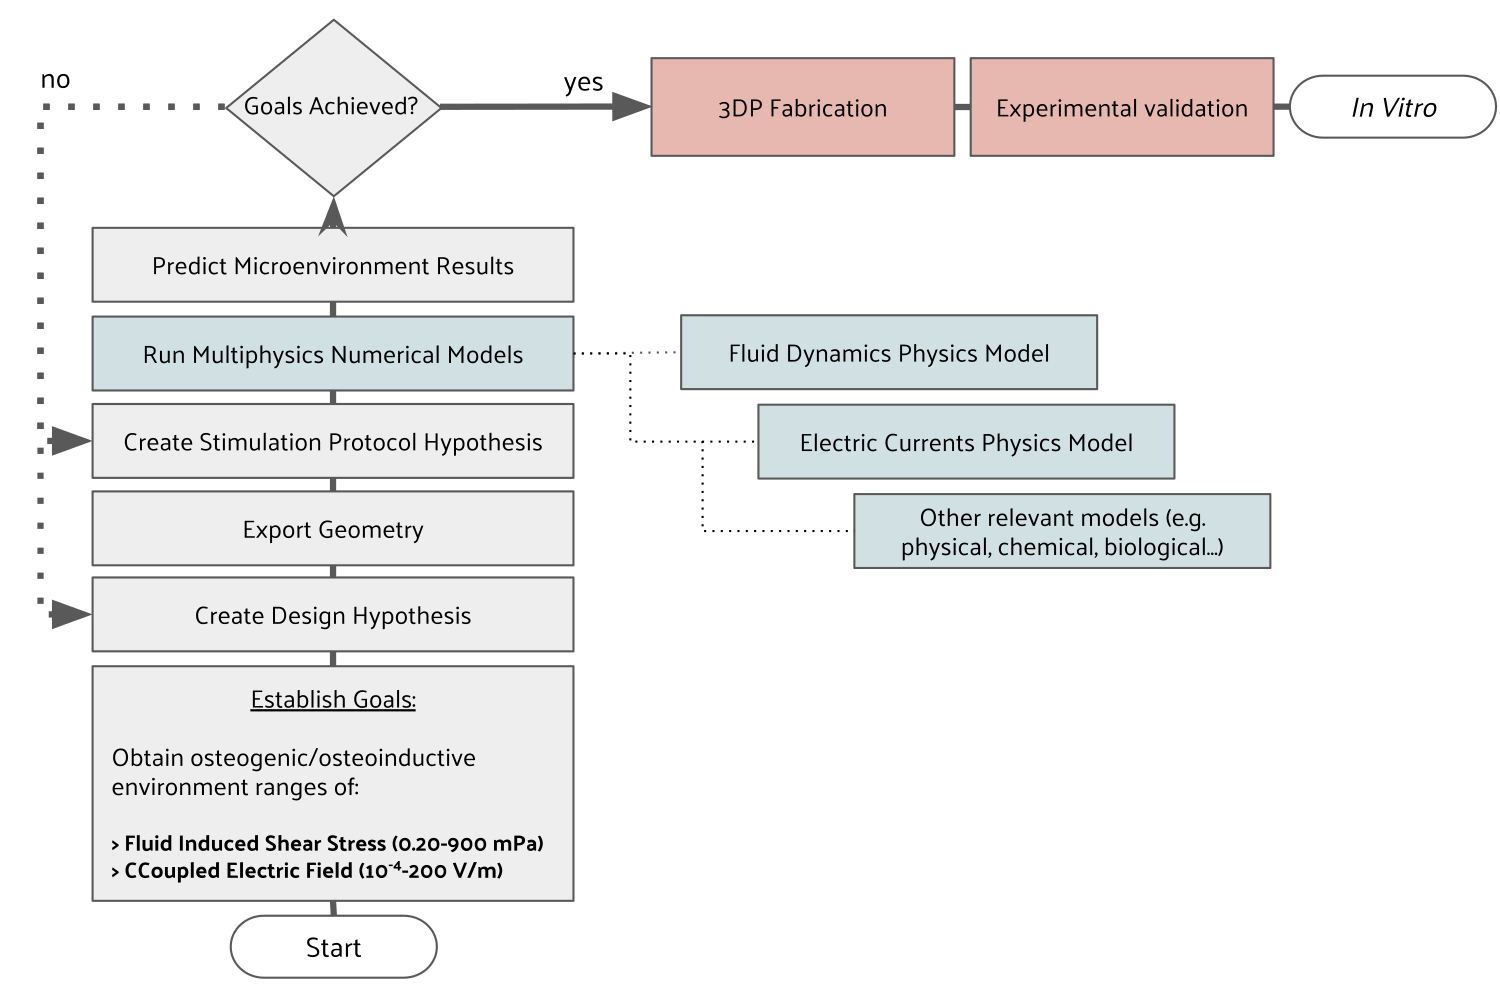
\includegraphics[scale=0.8]{./figures/Figure_6d4}}
\caption{Decision tree used to iterate between \acs{CAD} design and stimulation protocol hypotheses until \acs{FEM} predictions matched an intended microenvironment.}
\label{figStrategy}
\end{figure}

\begin{sidewaysfigure}
\makebox[\textwidth][c]{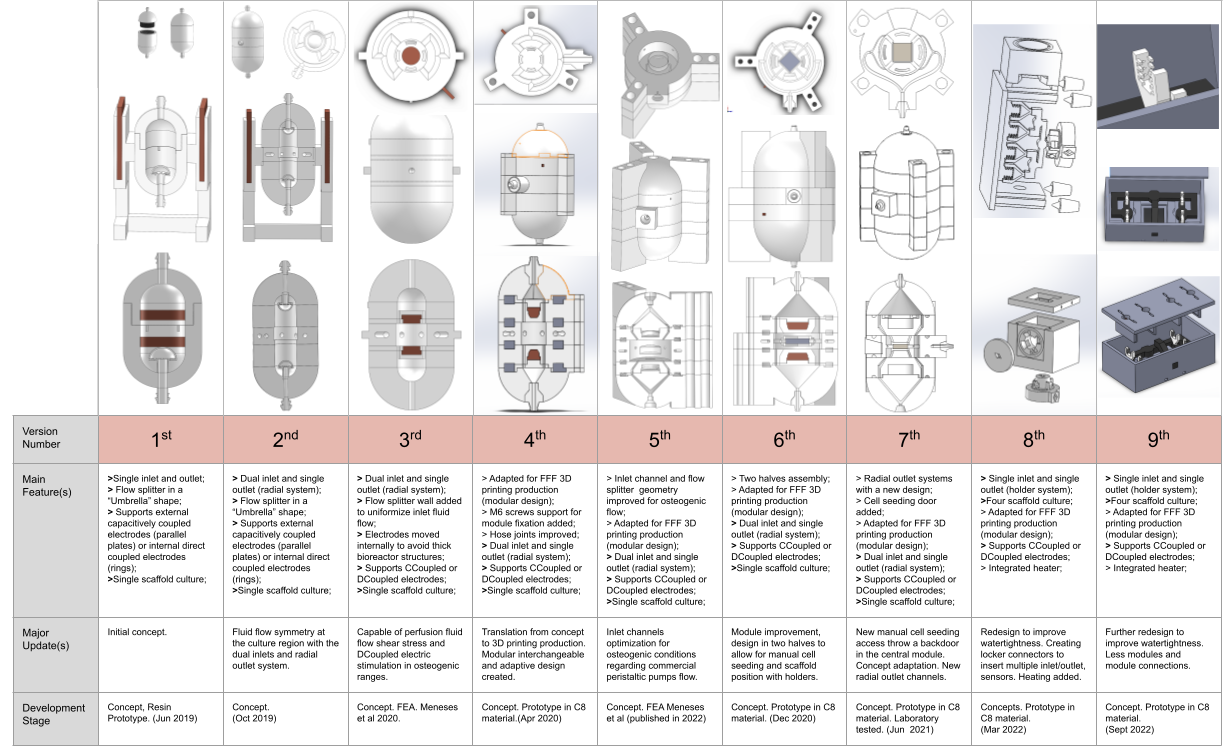
\includegraphics[scale=0.45]{./figures/Figure_6d4b}}
\caption{Development timeline of the bioreactor until the 9\textsuperscript{th} version used as the starting point for the bioreactor update presented in the current chapter.}
\label{figStory}
\end{sidewaysfigure}


\subsubsection{Defining the bioreactor system development goals}
The starting point for this design was a previously developed bioreactor concept \cite{Meneses2020-dx, Meneses2022-rx}. This design was progressively modified to integrate multiple actuators and sensors while preserving the ability to be entirely \acs{3D} printable (Figure \ref{figStory}). Culture medium volume usage was minimized, and sensor probes were included for online monitoring (e.g., pH, dissolved oxygen, temperature).

Perfusion bioreactors allow reaching cell-seeded scaffolds with homogeneous nutritional supply while removing waste products effectively, favoring appropriate cell metabolic activity \cite{Shakeel2013-vo, Gaspar2012-uz}. Also, the induced fluid flow shear stress can simultaneously act as a mechanical stimulus to promote improved responses in some cellular lines (bone cells included). Due to these two attributes, perfusion technology was selected for this development to ensure proper osteogenic conditions of the microenvironment. We chose a wall shear stress range in agreement with those previously observed to produce osteoinductive effects for mesenchymal stem/stromal cells. We refer to the osteoinductive ranges of 1.47-24 \unit{\milli\pascal} \cite{Vetsch2017-zd} and 0.20-13.35 \unit{\milli\pascal} \cite{Yamada2021-qf}. We emphasize that the resultant wall shear stress range is a product of the bioreactor-generated fluid flow characteristics, being also influenced by the scaffold properties, including its geometry and surface topology.

The other technical decision was to select adequate electrical stimulation technology for \textit{in vitro} cultures. Evidence of \acs{EF} technologies to support osteogenic processes has built up over the last decades and is extensively reviewed by Nicksic \textit{et al.} \cite{Nicksic2022-jy}. We decided on \acs{CCoupled} systems, since these ensure the delivery of a pure \acs{EF} stimulation without faradaic byproducts or an accompanying magnetic field. \acs{CCoupled} electrodes were fabricated from indium tin oxide coated polyethylene terephthalate (ITO PET) films (33x18 \unit{\milli\meter}), with a 175 \unit{\micro\meter}-thick polyester film coated with indium tin oxide (60 \unit{\ohm}/sq) that was glued with polydimethylsiloxane (PDMS) to a 3D printed structure. Regarding \acs{CCoupled} stimulation, the system will be designed to deliver an \acs{EF} with a wide range of magnitudes, considering the values previously reported of \num{1.0d-5} to \num{1.3d+3}\unit{\volt\per\meter} \cite{Fitzsimmons1986-ks, Korenstein1984-qb}, using a frequency of 60 \unit{\kilo\hertz} as applied by other previous \acs{CCoupled} works addressing bone regeneration \cite{Brighton1992-gg, Stephan2020-qh}.


\subsubsection{Creating geometrical design hypotheses}
All bioreactor and scaffold parts were designed with SOLIDWORKS (2018 Student Edition, Dassault Sistèmes), a parametric \acs{CAD} software. Two scaffold geometries were selected from the literature as an example to apply the described development methodology (Figure \ref{figParts}a, \ref{figParts}b). Our selection criteria were to consider scaffold geometries actively used in bone tissue engineering research, capable of matching the mechanical properties of cortical or trabecular bone formations to some extent. 

The first scaffold geometry selected is from Hayashi \textit{et al.} work \cite{Hayashi2019-qx, Hayashi2020-fr, Hayashi2022-oa, Shibahara2022-kj}, consisting of a honeycomb structure scaffold for bone regeneration, made from carbonate apatite to resemble natural human bone mineral composition. Their studies tested different macropore and micropore volumes, demonstrating that high interconnectivity and uniformity of channels enable scaffolds to maintain high mechanical properties and osteogenic ability while being suitable to be applied as implants for weight-bearing areas \cite{Hayashi2019-qx, Hayashi2020-fr}. This honeycomb scaffold structure was produced by extrusion molding, with a reported Young’s moduli of 23 \unit{\giga\pascal} \cite{Hayashi2020-fr}, higher than the usual Young’s moduli value for cortical (18-21 \unit{\giga\pascal}) or trabecular (10-15 \unit{\giga\pascal}) bone formations \cite{Morgan2018-pv}, but with the potential to be tailored by porous structures design to mimic mechanical properties of bone structures. The \acs{CAD} geometry of the honeycomb structure scaffold was considered with an external envelope volume of 10.2x10.2x3.0 \unit{\milli\meter}, a truss size of 250 \unit{\micro\meter} and a macropore size of 300 \unit{\micro\meter}. 

The second scaffold geometry selected is a regular orthogonal scaffold that, when produced from ceramic materials, such as biphasic calcium phosphate \cite{Touri2018-jw} or lithium-calcium-silicate crystal \cite{Chen2019-ap}, has reported properties similar to native bone minerals. The \acs{CAD} geometry of the orthogonal scaffold presents an external envelope volume of 10.0x10.0x2.75 \unit{\milli\meter}, while maintaining the geometrical relations and dimensions reported by Touri \textit{et al.} \cite{Touri2018-jw}, with a filament diameter and pore size of 500 \unit{\micro\meter}. Due to typical 3D printing fabrication constraints and to ease numerical models, a filament superposition of 10 \% and round fillets of 0.02 \unit{\milli\meter} diameter were added to each orthogonal intersection.


\begin{figure}
\makebox[\textwidth][c]{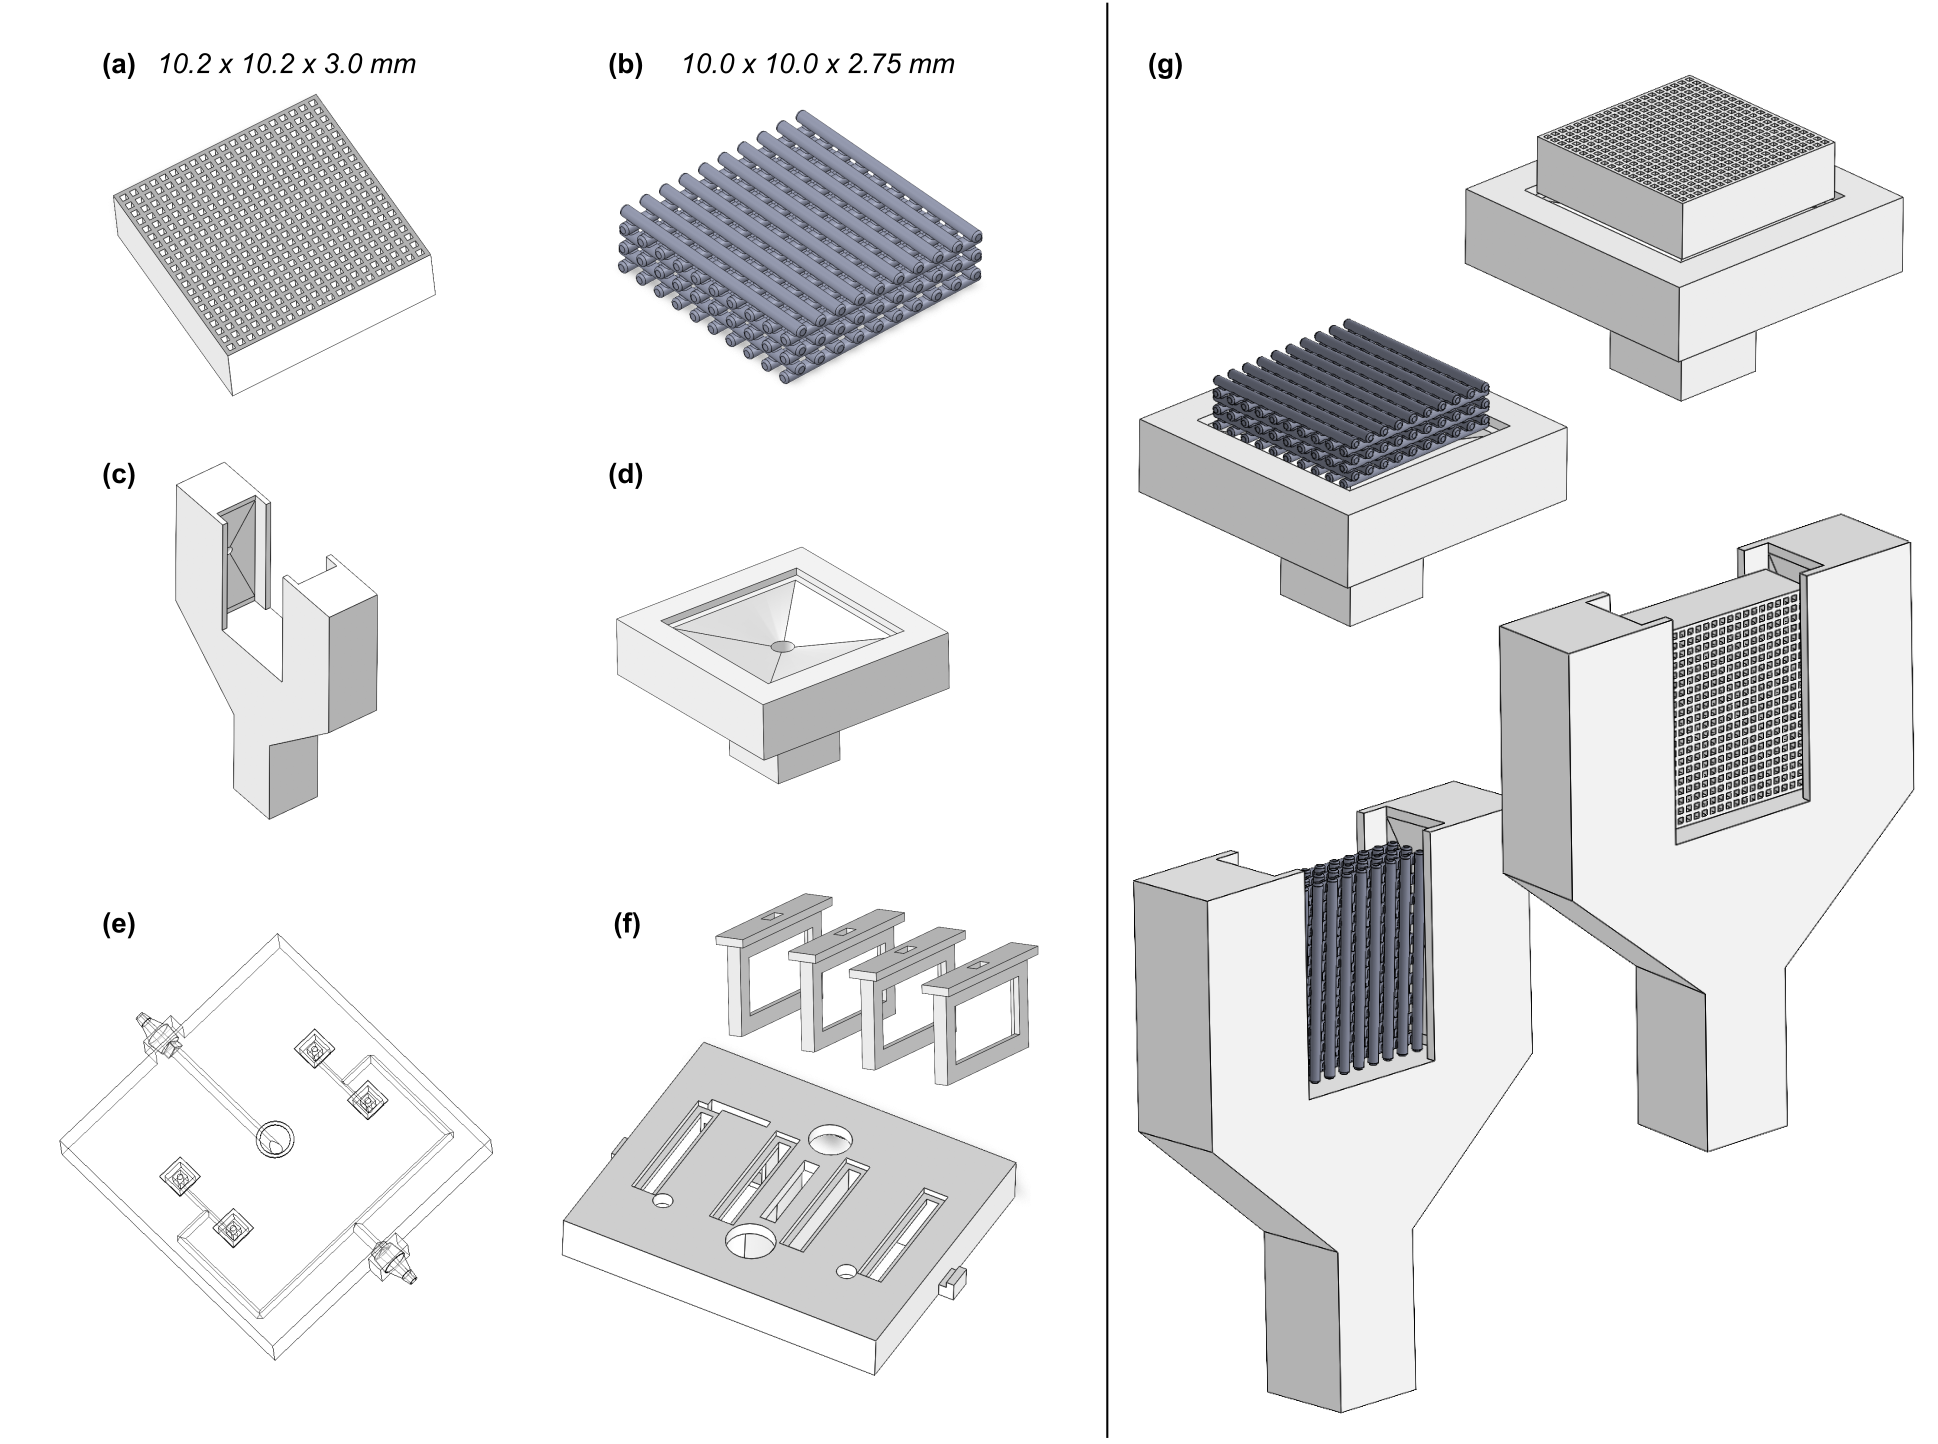
\includegraphics[scale=0.6]{./figures/Figure_6d5}}
\caption{Geometrical design hypotheses considered. (a) Honeycomb scaffold structure; (b) Orthogonal scaffold structure; (c) Vertical scaffold holder; (d) Horizontal scaffold holder; (e) Outlet channel network; (f) Support for CCoupled electrodes; (g) Combinations of scaffold and holder considered for simulations.}
\label{figParts}
\end{figure}


In addition to the scaffold design hypothesis, two versions of scaffold holders were conceived to provide support in different positions (vertical vs. horizontal), also incorporating different outlet flow channels (Figure \ref{figParts}c, \ref{figParts}d). The reason for this holder hypothesis was to provide different fluid flow characteristics (one bottom outlet vs. two lateral outlets), and also, since the CCoupled system is mounted laterally, the created holder hypothesis allows testing two electric stimulation configurations. To connect each of the bioreactor's four scaffold holders to the outlet peristaltic tube, a channel network (Figure \ref{figParts}e) was designed to guarantee that, at every channel split, the sum of section areas of the child branches is equal to the section area of the parent branch, condition necessary to minimize flow velocities loss, since it divides the outlet flow equally among all supported scaffolds. Regarding the \ac{CCoupled} system, since stimulation amplitude, waveform, and duration are the most determinant parameters for the \ac{CCoupled} effects, all geometrical variations of electrode number, position, or size were not considered in this work, being described elsewhere \cite{Tandon2008-jg}. Thus, the delivery range of the \acs{EF} in this work was varied only by changing the input waveform of the stimulation protocol. The electrodes for the \ac{CCoupled} system were placed in parallel positions and equidistant from the scaffold center, 22 \si{\milli\meter} apart, in such a way that each electrode pair will stimulate two side-by-side scaffolds (Figure \ref{figParts}f). 

The decision to have four scaffolds per bioreactor was to increase statistical power in the experimental condition, being a common practice in \acs{TE} to replicate the same condition in a high number of samples ($N>3$) \cite{Pollard2019-tz, Silva2020-dc}. To avoid unnecessary simulations and decrease computational effort, the proposed work was separated into two blocks: 1) obtain the outlet channel network design that minimizes the fluid flow velocity loss; 2) all combinations of scaffolds and holders designs were considered, resulting in four models that were analyzed with fluid flow and \acs{EF} simulation studies. The combination of geometries and protocol which predictably results in the closest conditions to an osteogenic microenvironment were selected for fabrication and validation.


\subsubsection{Setting simulation input parameters}
Each protocol was selected considering the maximum output of the available lab equipment (electric signal source and peristaltic pump), guaranteeing that the highest magnitudes possible for the available lab equipment were obtained for each stimulation condition at the cell culture chamber. Once determined the bioreactor-generated microenvironments for the maximum equipment's output, we established our working baseline: the peristaltic pump flow rate was set to the maximum continuous outlet flow of 50 \unit{\milli\liter\per\minute}, mounted with a 2.79 \unit{\milli\meter} internal diameter peristaltic tube (0.328 \si{\meter\per\second} at the peristaltic tube end); the CCoupled input waveform generator was set to its maximum amplitude of 10 \si{\volt}\textsubscript{p-p} for a sinusoidal wave with a frequency of 60 \unit{\kilo\hertz}. Both stimulation protocol parameters were considered as inputs for the developed numerical models.


\subsubsection{Multiphysics numerical simulations}
Each designed part was exported to the \acs{STEP} file format, allowing it to be imported and post-processed by COMSOL Multiphysics \acs{FEM} software (version 5.2a, www.comsol.com). Meshing was performed with the physics-controlled mesh and fine options. These options translated to meshes made from free tetrahedral elements with an average element quality of 0.68. Further mesh characterization data is available in the COMSOL reports, downloadable in an online repository (https://doi.org/10.5281/zenodo.7695700). Meshes were constructed with a high number of nodes to guarantee mesh-independent results (computable by the processor AMD Ryzen 7 5700G 8-Core 3.8GHz c/ Turbo 4.6GHz 20MB SktAM4). Two COMSOL physics interfaces were applied for each stimulation mode. For fluid flow shear stress calculations, \acs{CFD} stationary studies were conducted with the single phase Laminar Flow physics interface, which solves the Navier-Stokes equations for the conservation of momentum and the continuity equation for the conservation of mass. The cell culture medium was considered as an incompressible Newtonian fluid, with viscous material properties similar to water, as applied by Hidalgo-Bastida \textit{et al.} \cite{Hidalgo-Bastida2012-tp} and in our previous works \cite{Meneses2020-dx, Meneses2022-rx}. Outlet channel network flow models were imposed with an outlet velocity boundary condition of 0.328 \unit{\meter\per\second} applied to the peristaltic tube connector, and a standard atmosphere pressure (\num{1.01d5} \unit{\pascal}) inlet boundary condition applied to the scaffold holder connector channel. Flow models for scaffold and holder combinations were enclosed by a cylindrical volume with a radius of 20 \unit{\milli\meter} and a height of 30 \unit{\milli\meter} to represent a part of the culture medium domain inside the bioreactor chamber. The atmospheric pressure inlet boundary condition was considered in all surrounding cylindrical surfaces. In contrast, a single outlet boundary condition was added to the exit surface of the scaffold holder channel (designed with equal dimensions for both holder options). The scaffold holder outlet boundary condition was defined with the average velocity magnitude value (0.120 \unit{\meter\per\second}) obtained from the first outlet channel network model solution.


\begin{table}
\caption{Material properties for numerical model domains.}
\bigskip
\footnotesize
\centering
\begin{tabularx}{350px}{l l} \toprule[0.15em]
\textbf{Material} & \textbf{Properties} \\ \cmidrule(l){1-2}

Osteogenic Culture Medium (37  \unit{\celsius}) & 
\begin{tabular}[c]{@{}l@{}}Electric conductivity: 1.5 \unit{\siemens\per\meter} \\
Relative permittivity: 80.1 \\
Kinematic viscosity: \num{6.89d-4} \unit{\pascal\second} \\
Density: \num{9.94d2} \unit{\kilo\gram\per\cubic\meter} \cite{Gabetti2022-hp}
\end{tabular} \\ \cmidrule(l){1-2}

Electrode - ITO part                                                                   
& \begin{tabular}[c]{@{}l@{}}Electric Conductivity: \num{1.0d6} \unit{\siemens\per\meter} \\ 
Relative permittivity: 1 \cite{ReviewMIT}
\end{tabular} \\  \cmidrule(l){1-2}

Electrode - PET part 
& \begin{tabular}[c]{@{}l@{}}Electric Conductivity: \num{1.0d-21} \unit{\siemens\per\meter} \\
Relative permittivity: 3 \cite{ReviewMIT} 
\end{tabular} \\ \cmidrule(l){1-2}

C8 (PLA composite) - bioreactor parts
& \begin{tabular}[c]{@{}l@{}}Electric Conductivity: \num{1.0d-21} \unit{\siemens\per\meter} \\
Relative permittivity: 2.7 \cite{Hegde2015-nd}
\end{tabular} \\ \cmidrule(l){1-2}

PCL - scaffold 
& \begin{tabular}[c]{@{}l@{}}Electric Conductivity: \num{1.0d-13} \unit{\siemens\per\meter}\\ 
Relative permittivity: 3.2 \cite{Hegde2015-nd}
\end{tabular} \\ \bottomrule[0.15em]
\end{tabularx}
\label{table61}
\end{table}


\acs{CCoupled} \acs{EF} stationary calculations were performed with the Electric Currents physics interface, solving a current conservation equation based on Ohm’s law using the scalar electric potential as the dependent variable, assuming the quasistatic approximation as applied by Budde \textit{et al.} \cite{Budde2019-qe} and in our previous studies \cite{Meneses2022-yk, Fernandes2022-lj}. Electric potential boundary conditions were added to the outer surfaces of electrodes, 5 \si{\volt} to the active electrode (corresponding to 10 \si{\volt}\textsubscript{p-p}), 0 \si{\volt} to the other electrode (ground). A frequency domain study was conducted at 60 \si{\kilo\hertz}.

Material properties of each domain were set according to Table \ref{table61} for simulated protocols. \ac{FEM} results were post-processed with COMSOL for each hypothesis, considering the envelope volume surrounded by the selected cell culture scaffold as the \acs{ROI}. C8 and PCL materials were considered based on our results from the pre-culture validation tests.

COMSOL reports were generated for each numerical study and are available for download in an open-source repository (https://doi.org/10.5281/zenodo.7695700), containing a detailed description of all the parameters required to replicate the numerical research, following a documenting standard for TE stimulation studies proposed by Budde \textit{et al.} \cite{Budde2019-qe}. The volumetric distribution of Reynolds number, fluid-induced shear stress, fluid flow overall velocity, and axial component velocity magnitude was analyzed for \acs{CFD} models. Fluid-induced shear stress was calculated from COMSOL shear rate and water dynamic viscosity at 37 \si{\celsius} (approximation valid for Newtonian fluids \cite{Wilson2018-ss}). For \acs{CCoupled} models, the volumetric distribution of \acs{EF} magnitude and integration of the resultant electric current was analyzed.


\subsection{Fabrication of the bioreactor, scaffold, and supporting systems}
All \acs{3D} printable parts selected for production from the design hypothesis were fabricated with proprietary \acs{C8} material (3D4Makers, Netherlands) and printed with an Ender 3 S1 Pro 3D FFF printer (Creality, China). The printer specifications were set accordingly with the \acs{C8} manufacturer datasheet (printing temperature: 210 \si{\celsius}, bed temperature: 50 \si{\celsius}, maximum printing speed: 35 mm/s). Connectors and other support parts were fixed and isolated with PDMS (Sylgard 184 Silicone Elastomer Kit, applied in a 10:1 (w/w) ratio of base to curing agent) and left to dry overnight. The perfusion system was developed based on commercially available peristaltic pumps (details on the original manuscript supplementary materials). Custom sensor circuits, firmware, and software interfaces were developed to communicate commands via Bluetooth protocol to the bioreactor (details on the original manuscript supplementary materials). The scaffold geometry predicted to ensure the most optimal microenvironment was selected and 3D printed with polycaprolactone (PCL) material and evaluated for structural/morphological properties by micro-computed tomography using a SkyScan 1174TM (Brucker, Kontich, Belgium). Blueprints with all fabrication instructions and required source files are described in the original manuscript supplementary materials and available for download in an open-source repository (https://doi.org/10.5281/zenodo.7695700).


\subsection{Pre-culture validation}
All \acs{3D}-printed parts and electronic systems were tested individually to guarantee proper functioning. A complete description of each validation test may be found in the original manuscript supplementary materials, which include watertight tests, electronics, and communication operational tests. Individual sensor outputs were validated against golden standard devices or standard solutions. Their predictions were compared with experimental measurements of the fluid flow velocity and total electric current that passes through the \acs{CCoupled} system to validate the fabricated designs and correspondent numerical models. Both perfusion and \acs{CCoupled} systems were tested independently of one another. Notably, the \acs{CCoupled} system designed to be mounted on the top of the developed bioreactor perfusion chamber was tested in a specifically designed support that matches its final configuration. ITO PET capacitive electrodes were mounted 10 \si{\milli\meter} apart (see Figure \ref{figValidation}), separated by culture medium.


\subsection{Cell viability and metabolic activity validation after bioreactor culture}
A preliminary cell culture validation was performed with the proposed bioreactor system using \acs{PCL} scaffolds seeded with Human osteoblast-like MG-63 cells (ATCC\textregistered CRL-1427\texttrademark) under fluid flow static conditions (without perfusion), with and without the application of the previously defined CCoupled stimulation protocol (sinewave amplitude from 5 \si{\volt} to -5 \si{\volt}, 60 \si{\kilo\hertz}, 1 hour per day). A complete description of the applied cell culture process is available in the original manuscript supplementary materials. Briefly, the entire bioreactor system was sterilized by means of ethanol 70\% washing followed by 1\% v/v antibiotic-antimycotic (Gibco\texttrademark) solution (prepared in Phosphate Buffered Saline (PBS)) washing (all the bioreactor parts and also on tubing through perfusion using the peristaltic pump) and by ultraviolet light exposure for 2 hours. Then, human MG-63 osteoblasts were seeded (200,000 cells/scaffold) on the 3D-printed \acs{PCL} scaffolds and cultured for 12 days in static conditions to promote the population of the whole scaffold structure. Then, the cell-seeded scaffolds were transferred to the fabricated bioreactors and cultured for 48 \si{\hour} (2 days inside the bioreactor placed inside an incubator at 37 \si{\celsius} and 5\% CO\textsubscript{2}). Three experimental groups were created to evaluate cell viability and metabolic activity. A control group comprised cell-seeded scaffolds cultured on a well-plate static culture. Two test groups were formed of cell-seeded scaffolds cultured in the proposed bioreactor static culture with/without electric stimulation ($N=4$). Perfusion conditions were not considered for preliminary tests to allow better comparison with cell plate standard culture and with reported experimental studies of electromagnetic stimulation of Human osteoblast-like MG-63 cells, also performed under static medium conditions. Cell viability was assessed with a LIVE/DEAD staining (Life Technologies), and the metabolic activity was evaluated via the Alamar Blue assay (Thermo Fisher Scientific), both protocols are available in the original manuscript supplementary materials. 


\subsection{Statistical analysis}
Statistical analysis of the data was performed by one-way ANOVA, followed by a Tukey post-hoc test using the GraphPad Prism 7.0 software (GraphPad, San Diego, CA, USA). Data were considered statistically significant when the p-values obtained were less than 0.05 (95\si{\percent} confidence intervals, $p<0.05$). 


\section{Results}

\subsection{\textit{In vitro} cytotoxicity tests}
Candidate materials for the fabrication of the bioreactor platform were evaluated in terms of their cytotoxicity effect using an L929 fibroblast cell line and following the ISO 10993-5 standards as described in the Methods section (Figure \ref{figCito}). Using a one-way ANOVA with no corrections for multiple comparisons (Fisher’s test), it was possible to observe that \acs{PCL} and \acs{C8} materials do not present any response compared to the negative control ($p>0.05$). Despite the statistical differences visible in Figure \ref{figCito}, ISO standards state that only materials with cell viabilities less than 70\% are considered cytotoxic. This way, it is possible to affirm that from all materials tested \acs{PCL} (90.48 $\pm$ 3.88 \%), PPSU (82.57 $\pm$ 6.45 \%), ABS (79.05 $\pm$ 4.16 \%), C8 (88.67 $\pm$ 4.69 \%), PETG (78.63 $\pm$ 5.69 \%) and PEEK (81.84 $\pm$ 12.39 \%) are not cytotoxic materials. The remaining material PA (75.73 $\pm$ 10.47 \%) had some samples with cell viabilities below 70 \%, and according to the applied criteria, it was excluded from the not cytotoxic materials list. 

\begin{figure}
\makebox[\textwidth][c]{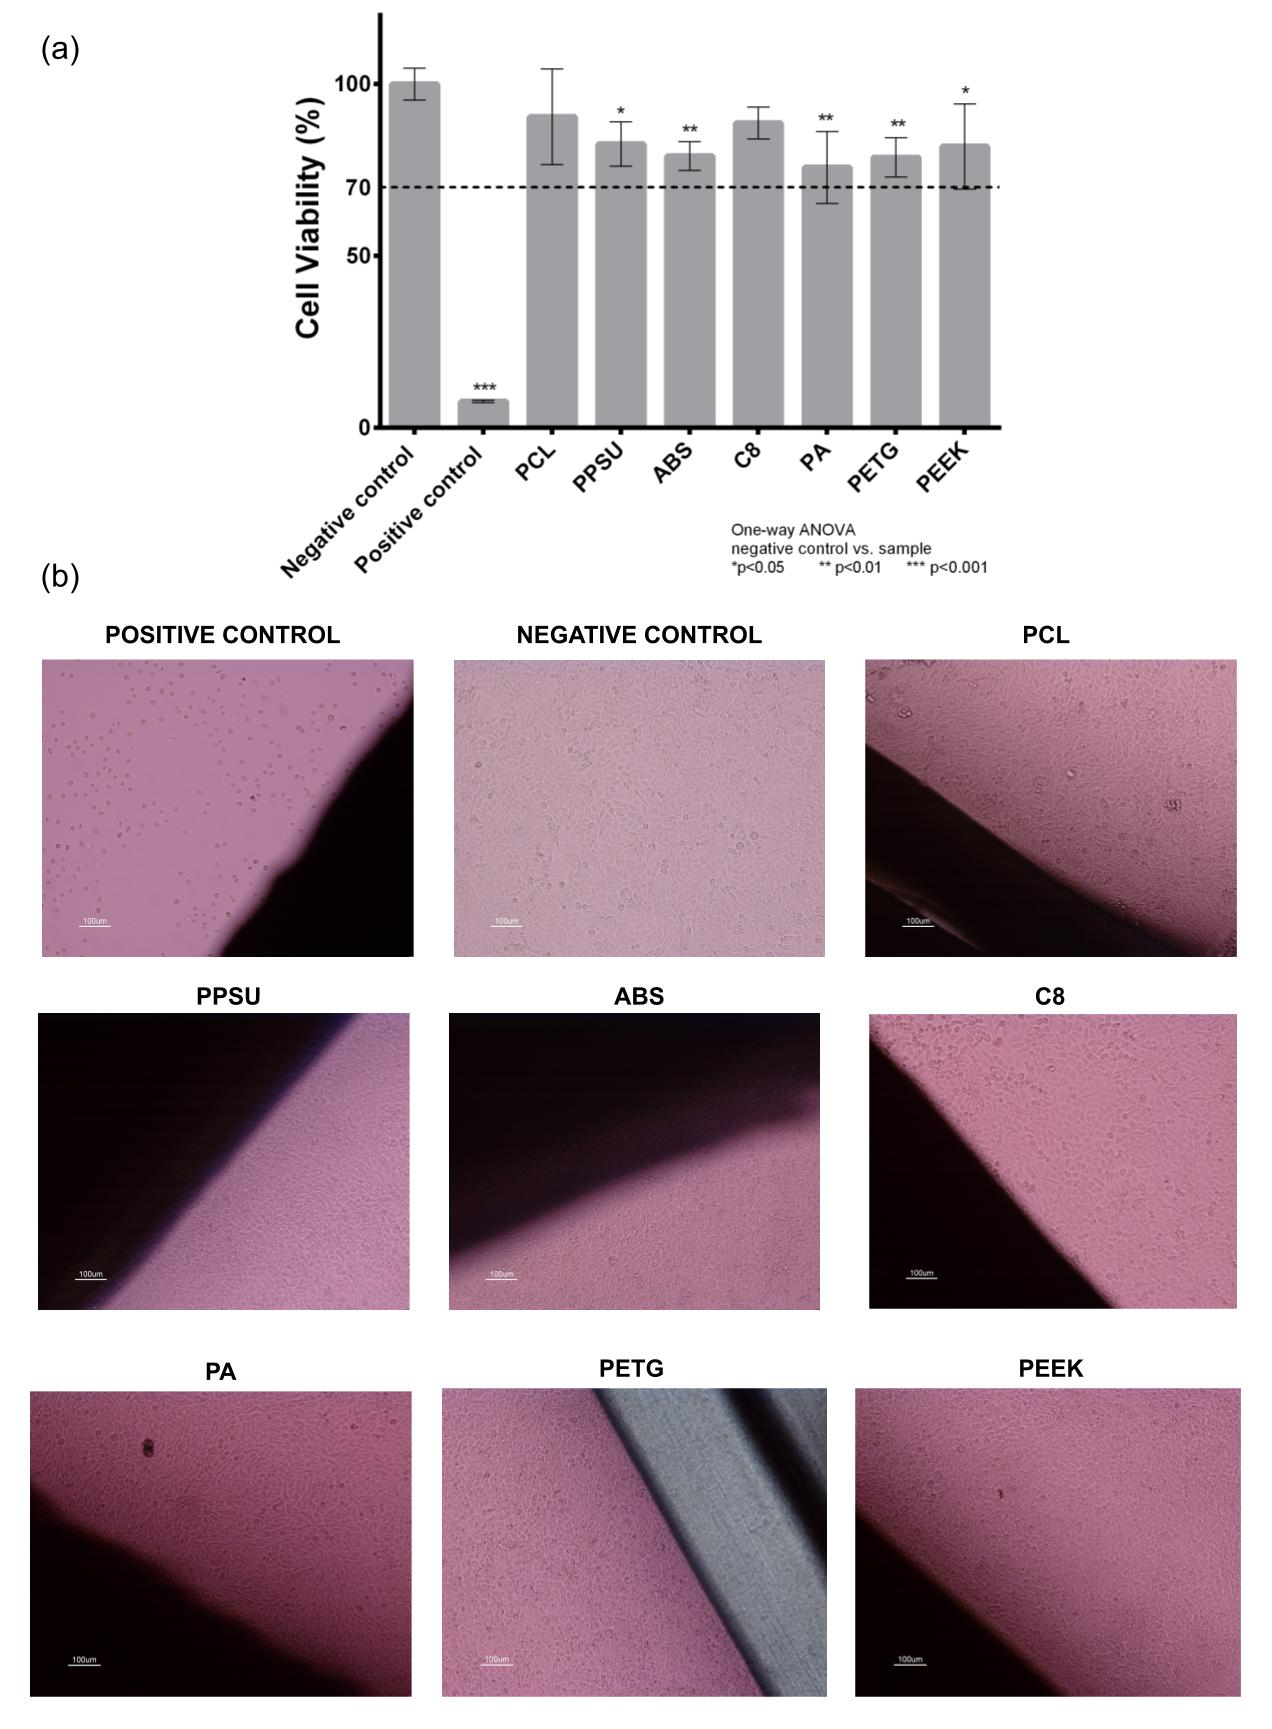
\includegraphics[scale=0.25]{./figures/Figure_6d3}}
\caption{{Cytotoxicity assay with L929 mouse fibroblast according to ISO 10993-5 standards: (\textbf{a}) indirect contact (MTT protocol); (\textbf{b}) direct contact (digital images of the material samples and the negative and positive controls, fresh culture medium and Latex, respectively). A one-way ANOVA with no corrections for multiple comparisons (Fisher’s test) statistical analysis was performed using GraphPad Prism6.}}
\label{figCito}
\end{figure}


\subsection{Bioreactor design based on model-driven decisions}
This section presents results from numerical models, starting from the predicted generated microenvironment for each bioreactor, scaffold, and holder design hypothesis considered. Then, after selecting the design that predictably generates the most osteogenic microenvironment, results from experimental validation using the developed systems are presented and compared with predictions from their numerical models. Finally, \textit{in vitro} preliminary cell culture validation results are described regarding cellular viability and metabolic activity. 


\subsubsection{Predicted bioreactor microenvironments}
The developed bioreactor design (Figure \ref{figExploded}) minimizes the culture medium volume to 45 \unit{\cubic\centi\meter}, a decrease of 91\% from our previous bioreactor version, reducing significantly culture media-related costs. This volume reduction also impacted the channel network design. From \acs{CFD} analysis, we estimated a surface average velocity magnitude of 0.120 \unit{\meter\per\second} at each scaffold holder connector channel, corresponding to an outlet velocity of 0.328 \unit{\meter\per\second} for the maximum peristaltic pump flow rate of 50 \unit{\milli\liter\per\minute} (hose connector section area of 0.0254 \unit{\square\centi\meter}). The \acs{CFD} velocity profiles of all four scaffold holder connector channels were predicted to be equal, according to the construction design strategy adopted and explained in the methods section.


\begin{figure}
\makebox[\textwidth][c]{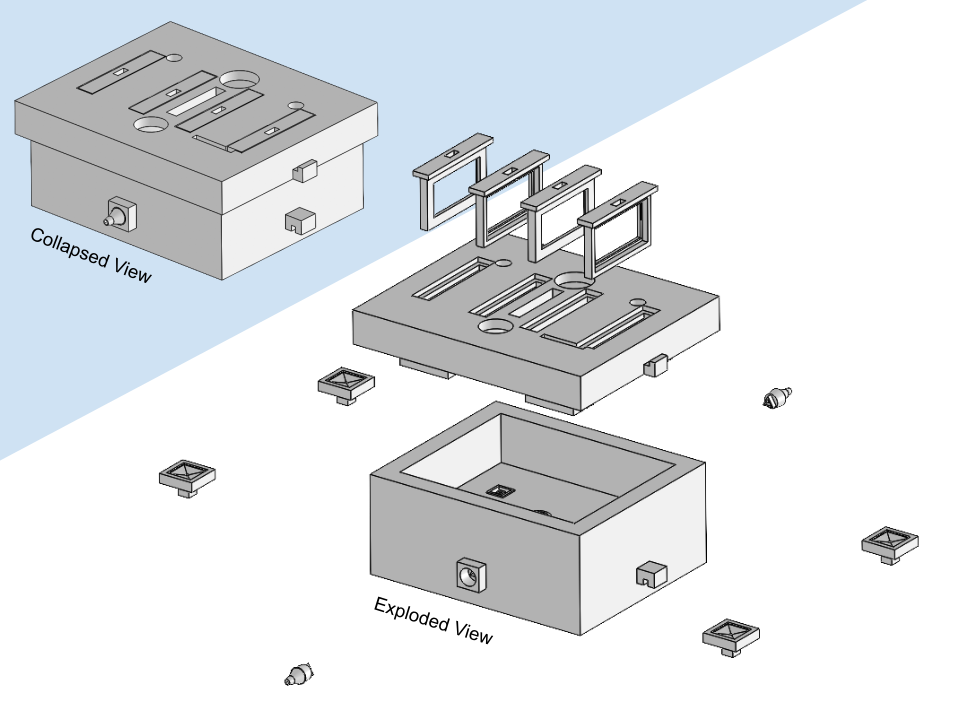
\includegraphics[scale=0.5]{./figures/Figure_6d6.png}}
\caption{Illustration of the developed bioreactor and its components. Left upper corner: assembled collapsed view. Right bottom corner: exploded view. Only the horizontal scaffold holders option is represented.}
\label{figExploded}
\end{figure}


The two holders and scaffold designs were combined into four design hypotheses (a-c, a-d, b-c, and b-d are all created combinations as shown in Figure \ref{figParts}). For the outlet's perfusion velocity (at maximum peristaltic pump flow rate), the Reynolds number predicted was within the laminar flow limits ($<0.1$ \cite{LaNasa2014-hl}) for all design combinations. Histograms for the volume distribution of the fluid-induced shear stress are presented in Figure \ref{figWSS}.

The holder at the horizontal position originates a broader shear stress spectrum for both selected scaffold geometries. Once we are using the maximum peristaltic pump flow rate, this means that the horizontal holder configuration is the only one that may allow us to tune the fluid-induced shear stress by decreasing/increasing the peristaltic pump flow rate debit if required. In in the original manuscript supplementary materials Figure S8a, the impact of changing the peristaltic pump flow rate is exemplified, an action that will allow fitting the fluid flow-induced shear stress to a recommended cellular range of mechanical stimulation. Even considering the outcomes of the considered maximum peristaltic pump flow rate, at cell culture ROI, if both scaffold designs were placed in the horizontal holder, both would be able to generate a microenvironment inside the reported osteogenic ranges, 0.0015-0.024 \unit{\pascal} \cite{Vetsch2017-zd}, 0.00020-0.013 \unit{\pascal} \cite{Yamada2021-qf}, (Figure \ref{figWSS}, original manuscript supplementary Figure S8b). It is observable in the numerical predictions (Figure \ref{figWSS}), for all considered scaffold and holder combined geometries, that most of the volume fractions values occur within a range from 0 to 0.1 \unit{\pascal}. Remarkably, the horizontal holder and orthogonal scaffold combination show most of the predicted volume fractions in a range of 0 to 0.02 \unit{\pascal}, already inside the reported osteogenic ranges.


\begin{sidewaysfigure}
\centering
\includegraphics[width=\textwidth]{./figures/Figure_6d7.png}
\caption{Relative volumetric distribution of the fluid-induced shear stress (in units of \unit{\pascal}) for all combinations of selected scaffolds and holders, predicted by the \acs{CFD} numerical model at the culture \acs{ROI}. The maximum peristaltic pump rate of 50 \unit{\milli\liter\per\minute} was considered at the outlet. The volume axis refers to the number of node occurrences of the correspondent shear stress in the \acs{ROI}, normalized to its peak value.}
\label{figWSS}
\end{sidewaysfigure}


The horizontal holder was then selected since it provided optimal fluid-induced shear stress conditions for osteogenic effects, and the predicted volumetric distributions of the electric field for this holder and the established protocol were compared (see methods section). 

When comparing both scaffold geometries placed upon the horizontal holder (Figure \ref{figEF}), the orthogonal scaffold is the one with a higher \acs{EF} magnitude predicted at culture \acs{ROI}, with an average value of 0.118 \unit{\volt\per\meter}. In comparison, the honeycomb scaffold has an average electric field magnitude of 0.035 \unit{\volt\per\meter}. The observed non-uniformity of the electric field follows previously reported studies \cite{Meneses2021-nd}. These prediction results are caused by the presence of a scaffold structure that introduces an obstacle to the flow of charges (original manuscript supplementary Figure S8b). The effect of the scaffold's presence on the electric field in the surrounding culture medium is mainly determined by its geometry and by the difference in electrical conductivity of the scaffold materials and surrounding culture medium. Combining the horizontal holder with the orthogonal scaffold thus allows for a broader range of multimodal stimulation (simultaneous fluid-induced shear stress and \acs{EF}). For this reason, this was the hypothesis selected for fabrication and subsequent validation.



\begin{sidewaysfigure}
\centering
\includegraphics[width=\textwidth]{./figures/Figure_6d8.png}
\caption{Relative volumetric distribution of the electric field magnitude (\unit{\volt\per\meter}) for all combinations of scaffolds and holders when subjected to the \acs{CCoupled} stimulation (sine wave, 60 \unit{\kilo\hertz}, 10 \unit{\volt}p-p). All data was obtained from frequency domain \acs{EF} numerical model predictions at the culture \acs{ROI}. The volume axis refers to the number of node occurrences of the correspondent \acs{EF} magnitude in the \acs{ROI}, normalized to its peak value.}
\label{figEF}
\end{sidewaysfigure}


\subsection{Fabrication and pre-culture validation}
Bioreactor parts, selected scaffold, and holder structures were \acs{3D} printed as described in the methods section. Systems electronics were assembled, and probes were inserted into their established positions inside the bioreactor. Pre-culture tests were performed as described in the methods section (further details in original manuscript supplementary materials). The bioreactor produced in \acs{C8} composite material and externally coated in PDMS presented no water leaks in the watertight test after 24 \si{\hour} at 37 \unit{\celsius}, external or internal (infill space). The 24 \si{\hour} continuous perfusion test was successful, \textit{i.e.} the developed perfusion system sustained the required liquid level for that period. The individual operation of each applied sensor was confirmed in terms of stability and performance. Micro-computed tomography applied to the produced \ac{PCL} orthogonal scaffold samples revealed a mean pore size of $490 \pm 30$ \unit{\micro\meter} and a mean filament diameter of $518 \pm 30$ \unit{\micro\meter}, which are within the values originally established for both properties. 

Perfusion velocity measurements corresponded well to the numerical model predictions for the fluid flow at the bioreactor culture chamber without scaffold structures, as seen in Figure \ref{figValidation}(a). The two-time points, 13 \si{\second} 042 \si{\milli\second}, 16 \si{\second} 005 \si{\milli\second}, correspond to a yellow dye movement of 7 \si{\milli\meter} on top of the scaffold holder, which results in a mean velocity of 2.36 \si{\milli\meter\per\second}, following the numerical prediction (2-3 \si{\milli\meter\per\second}) for the same region and conditions. 

Regarding the \acs{CCoupled} stimulation system, the numerical model predicts an \acs{EF} of \num{0.095} \si{\volt\per\meter} and an electric current of \num{3.21d-5} \si{\ampere} at the testing setup (using the material properties and values from Table \ref{table61}). The experimental value of the electric current on the testing setup was \num{2.43d-5} \si{\ampere} (measured across a resistor with \num{21.89} \si{\kilo\ohm}, Figure \ref{figValidation}(b)). Using the developed \acs{FEM} model and setting a floating potential boundary condition for these two currents, the model predicts an electric field magnitude of 0.072 \si{\volt\per\meter} (for 24 \si{\micro\ampere}) and 0.095 \si{\volt\per\meter} (for 32 \si{\micro\ampere}). A numerical prediction with a 24\% difference for the same region and conditions, that at this scale could have been caused by model imprecisions in material properties. The developed \acs{CCoupled} stimulation system model neglected the \num{21.89} \si{\kilo\ohm} resistor used to perform the measurement currents. If accounted for (by means of a circuit terminal boundary condition), it would drop the predicted electric field magnitude to 0.094 \si{\volt\per\meter} (with a predicted current of \num{31.8} \si{\micro\ampere}). Despite being neglected in the developed system model, due to its narrow impact, adaptations of this \acs{CCoupled} stimulation system that change any of its main components should reconsider the measurement resistor impact.    


\begin{figure}
\centering
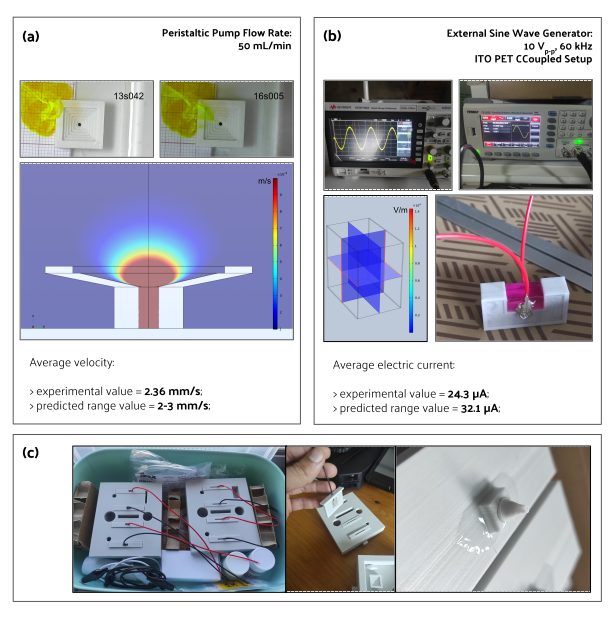
\includegraphics[width=\textwidth]{./figures/Figure_6d9.png}
\caption{Pre-culture validation of the fabricated perfusion bioreactor and its \acs{CCoupled} system and comparison with the numerical model's predictions for (a) fluid flow velocity and (b) electric current generated. The \acs{EF} generated by the \acs{CCoupled} system validation setup was predicted to be uniform, with a value of 0.095 \unit{\volt\per\meter} at the culture medium region. (c) Photos from the assembled bioreactor, electrodes, and perfusion connectors.}
\label{figValidation}
\end{figure}


\subsection{\textit{In vitro} cell culture viability and metabolic activity validation}
The preliminary validation results of the fabricated perfusion bioreactor and its \acs{CCoupled} system showed an applied \acs{EF} magnitude volume average of 0.118 \unit{\volt\per\meter}, which does not appear to impact the viability of human MG-63 osteoblasts. High cell viability was observed with no evidence of cell death in all conditions, as shown in Figure \ref{figViability}. Nonetheless, a significant effect is observed for this cell line when comparing cell-seeded scaffolds cultured in 24-well plates versus the bioreactor (no perfusion condition), with the latter presenting inferior metabolic activity (Figure \ref{figMetabolic}) but maintaining high cell viability and spreading around the scaffold (Figure \ref{figViability}). Overall, the validation tests confirmed that the fabricated bioreactor design can support cell cultures without signs of cytotoxicity or reduced cellular viability.


\begin{sidewaysfigure}
\makebox[\textwidth][c]{\includegraphics[scale=1.0]{./figures/Figure_6d10.png}}
\caption{Results from the bioreactor preliminary human MG-63 osteoblasts cell culture viability tests performed with LIVE/DEAD staining at day 14 (after 3x \acs{CCoupled} stimulation and 48h bioreactor culture).}
\label{figViability}
\end{sidewaysfigure}

\begin{figure}
\centering
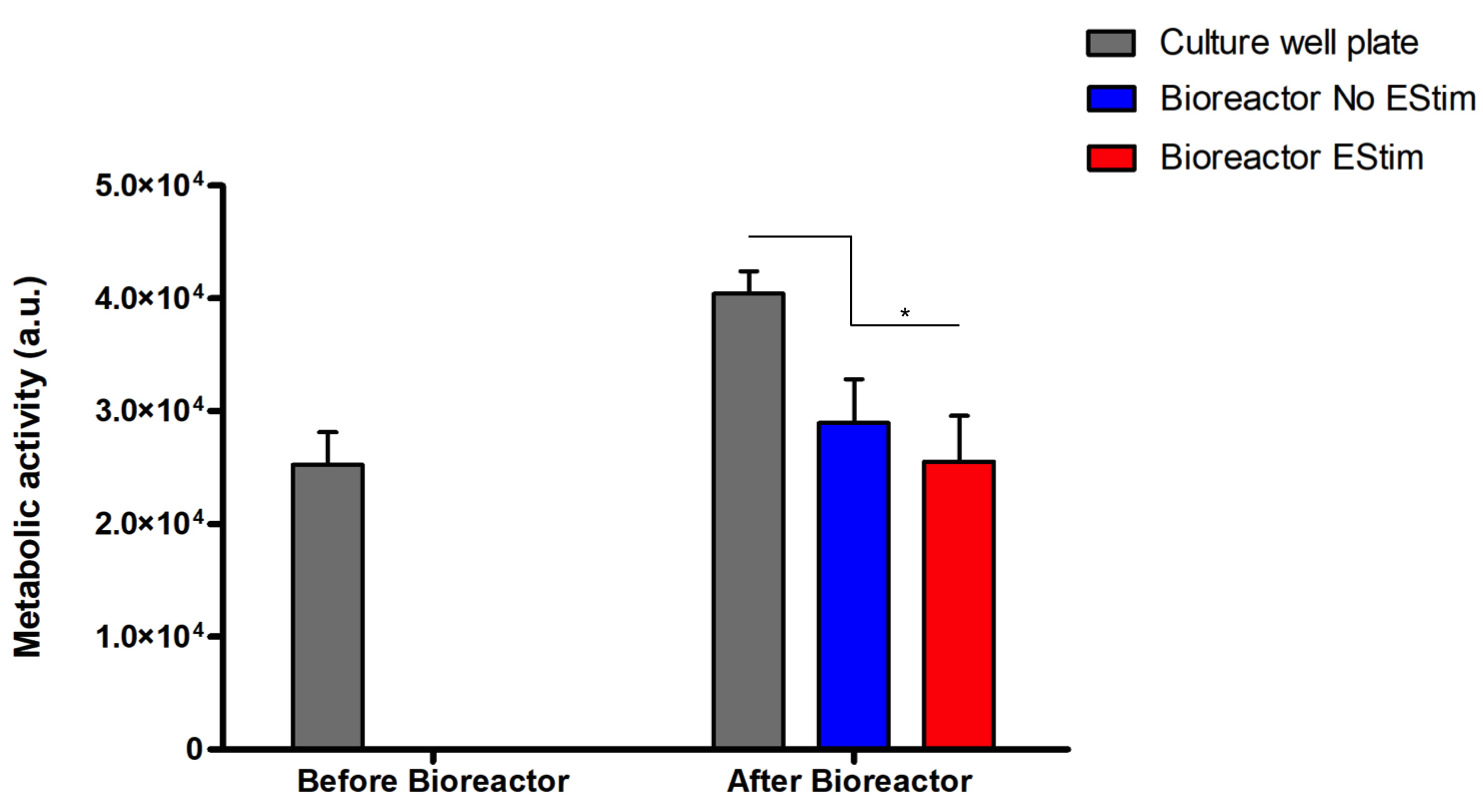
\includegraphics[width=\textwidth]{./figures/Figure_6d11.png}
\caption{Results from the metabolic activity of human MG-63 osteoblasts on a bioreactor preliminary static cell culture. Results present time points before (Day 12) and after bioreactor culture (Day 14) with/without \acs{CCoupled} stimulation. * account for significant differences $p<0.05$.}
\label{figMetabolic}
\end{figure}




\section{Discussion and limitations}
From a bird's eye view, the developed bioreactor design is one of many possibilities that can be obtained if considering different starting points, actuation strategies, and goals to be achieved. Nonetheless, the development strategy ensures that the produced design complies with the application of predetermined stimulation environmental conditions, even when applied simultaneously, like combined fluid-induced shear stress and \acs{EF} stimulation. 

\subsection{\textit{In vitro} cytotoxicity tests}
Accordingly, in the direct contact test, cells cultured in contact with all the materials presented normal fibroblast morphology with no evidence of any inhibition halo effect or cell death. According to the cytotoxicity test results, all candidate materials are suitable for our bioreactor additive fabrication. We picked \acs{C8} as the material of main interest for future design fabrication. \acs{C8} is a new material with good layer adhesion and surface quality, which are key features for perfusion flow. The \acs{C8} supplier datasheet reveals that this material has a higher tensile strength than ABS, resulting in improved mechanical characteristics, which are important for the overall robustness of the bioreactor to withstand the tightness of pressure chambers.


\subsection{Decisions on bioreactor fabrication}
We used numerical models to update the geometry or the stimulation protocol until established microenvironment properties were achieved. This iterative strategy is only possible if the resultant bioreactor design can be fabricated with high precision, a premise obtained through additive manufacturing technologies \cite{Gensler2020-in}. Various concepts of perfusion bioreactors \cite{Smith2018-he, Daneshgar2019-tu, Gabetti2022-hp, Birru2018-rj} have been \acs{3D} printed with stereolithography technology using class I biomaterial dental resin, while others have used fuse deposition modelling technology \cite{Rosser2018-zg, Schmid2018-rg, Raveling2018-gl}. A challenge with fuse deposition modelling 3D prints is to obtain leakproof components, since this process usually generates highly porous structures between filaments deposition. Different solutions were applied to overcome this issue. One approach was to cast an acrylonitrile butadiene styrene (ABS) part with a type of silicone rubber that cures at room temperature (commercially known as RTV silicone), creating a part mold and filling it with a two-part polyurethane casting resin \cite{Rosser2018-zg, Schmid2018-rg}. Another approach was to 3D print the bioreactor in ABS and waterproof it by treating its parts with an acetone vapor bath \cite{Raveling2018-gl}. In the present study, the bioreactor device was 3D printed, and afterward, all its 3D-printed pieces were coated with an external PDMS coating to achieve a watertight structure. Theoretically, it is possible to produce fuse deposition modelling leakproof parts without any added coating using larger nozzles and higher filament superposition. However, in a natural setting, this remains challenging due to small manufacturer imprecisions that occur during the printing process. Using an external coating allowed us to correct imprecisions that may have occurred during the 3D printing process.


\subsection{Bioreactor inner environment}
Some bioreactor-based strategies targetting bone regeneration are scaffoldless, like the one from Smith \textit{et al.} \cite{Smith2018-he} that uses a Kenzan micro-needle array; others support a single scaffold or single tissue sample \cite{Daneshgar2019-tu, Gabetti2022-hp, Schmid2018-rg, Rosser2018-zg, Birru2018-rj, Visone2018-sa}. Our design can support four scaffold structures under identical conditions in the same bioreactor. The operation concept behind our design is also flexible to expand to support even more scaffold structures.

The capability to monitor the fluid flow or electric phenomena in the presence of the scaffold structure and cellular content may be crucial to update and take more advantage of numerical models, extending their application into the monitoring and controlling of the cell culture microenvironment during the entire culture phase. Smith \textit{et al.} \cite{Smith2018-he} integrated a Doppler ultrasound imaging system to assess the flow characteristics inside the bioreactor culture chamber. Abasi \textit{et al.} \cite{Abasi2020-fn} proposed an electrical stimulation system that includes real-time monitoring of the response of a cellular membrane via AC electrical impedance spectroscopy. This design hypothesis may be fruitful in understanding electric changes in the cultured tissue. Our developed bioreactor uses commercially available sensors to perform real-time monitoring of pH, dissolved oxygen, and temperature fluctuations. However, there is still room for improvement regarding more accurate and less invasive procedures and/or miniaturized sensors.

Regarding multimodal stimulation approaches (fluid flow-induced shear stress and electromagnetic), the bioreactor designs from Gabetti \textit{et al.} \cite{Gabetti2022-hp} and Visone \textit{et al.} \cite{Visone2018-sa} are only two of the few examples of uni/bi-directional perfusion and simultaneous stimulation with a pulsed electromagnetic field. Visone \textit{et al.} \cite{Visone2018-sa} also introduced an original design that allows a microscopic observation of the cell culture without exposing it to an external environment. Our proposed bioreactor approach similarly allows the delivery of uni/bi-directional perfusion, alone or combined with an electric field stimulation system, conceived as capacitively coupled to induce a pure electric field to the cell cultures inside the bioreactor and avoid cell toxicity due to faradaic products that can occur in direct-coupled systems. Our current design capabilities can be further expanded with actuators to control temperature and O\textsubscript{2} / CO\textsubscript{2} gas concentrations, incorporating a system similar to the one described by Samokhin \textit{et al.} \cite{Samokhin2022-oy}.


\subsection{Bioreactor validation}
Once fabricated and before the introduction of \textit{in vitro} cell culture tests, the bioreactor was subjected to a pre-validation experiment to confirm if the conditions predicted in the numerical models are verified in the physical bioreactor system. Pre-culture validation results were in close correspondence with the experimental measures. Fluid flow velocity measurement was based on a video recording of a yellow dye wavefront movement, and the velocity was estimated using correspondent elapsed time between two known positions. This measurement was performed without a scaffold to improve the camera's field of view over the dye flow. The recorded fluid flow velocity (2.36 \si{\milli\meter\per\second}) matched the numerical predicted range for the same scaffoldless conditions at that same region (2-3 mm/s). Despite this agreement, more accurate techniques, like micro-particle image velocimetry \cite{Guastamacchia2022-bf} or ultrasound \cite{Smith2018-he}, could be applied to reconstruct velocity and shear stress fields in the presence of scaffold structures, allowing for comparison of CFD numerical models and experimental results with greater detail. \acs{EF} are difficult to measure directly, so we choose to determine their value by measuring the total electric current across a resistor in series with the CCoupled testing setup. A specially designed validation setup was built for the CCoupled system to spend less volume of culture medium, while keeping identical conditions to the cell culture chamber without any scaffold or holder structures. The developed numerical model of this testing setup predicted a current of \num{3.21d-5} \unit{\ampere}, higher than the measured value (\num{2.43d-5} \unit{\ampere}), but of the same order of magnitude. This slight overestimation may be caused by the material electrical properties adopted based on previous literature-reported values. This model should be further refined with electronic impedance spectrum characterization of the involved materials, since impedance may relate to the applied signal frequency \cite{10261_305757}. Natural bone streaming potentials are thought to be in the proximity of \num{0.39} $\pm$ \num{0.14} \si{\milli\volt} \cite{Qin2002-bn}, electric potentials that can be currently generated in the ROI using the developed CCoupled system by lowering the amplitude of the applied sinusoidal wave.

Pre-culture validation was essential to confirm that numerical model predictions and experimental measures obtained were in close agreement. This approach serves two primary purposes: first, differences can help improve both models and design/fabrication procedures; second, matching values increases the confidence in our pipeline for bioreactor design and fabrication. Thus, we recommend that future studies using numerical models to fine-tune the 3D design of bioreactors should include pre-validation assessments.


\subsection{Numerical modelling approaches}
Multiple studies on bioreactor concepts introduced numerical models to predict the applied microenvironment conditions. Usually, these studies applied \acs{CFD} models to empty chamber bioreactor digital designs to calculate flow regimes, velocity profile, and flow-induced shear stress \cite{Smith2018-he, Daneshgar2019-tu, Gabetti2022-hp, Rosser2018-zg, Schmid2018-rg, Visone2018-sa, Lim2019-gx}. Gabetti \textit{et al.} \cite{Gabetti2022-hp} also performed electromagnetic field simulations to predict the distribution of the delivered magnetic field, and Visone \textit{et al.} \cite{Visone2018-sa} performed an electric field estimation very similar to the one performed in our work. Compared with our modelling strategy, these previous studies did not modify the bioreactor design interactively to adjust microenvironment predictions, thus limiting microenvironment adjustments using only external manipulation. Also, these works did not include models with scaffold structures, which are widely used in \acs{TE} strategies and can powerfully shape fluid flow and electric field delivery. One improvement that may need to be addressed by future models is the need to introduce scaffold surface topology, since different scaffold surface properties will introduce local fluid flow-induced shear stresses that may be relevant in the generated biological response. Numerical models have commonly been used in isolation as alternatives to experimental measurements. However, with our approach, we demonstrate that it is a good practice to establish a VVUQ (verification–validation–uncertainty quantification) procedure when dealing with numerical models to cross-validate the model and bioreactor/scaffold fabrication before the cell culture studies phase.


\subsection{\textit{In vitro} cell culture tests}
Preliminary cell culture validation was performed with human osteoblast-like MG-63 cells, a cell type usually applied in osteogenic-related studies \cite{Ghanbari2023-du, Dehkordi2022-ku}. Although cell viability remained impaired, cell metabolic activity was affected when the scaffolds with seeded cells were transferred from the well plate to the bioreactor. The decrease in metabolic activity was further enhanced by the application of a low-intensity\acs{EF} (0.118 \unit{\volt\per\meter}), an effect also observed by Cohly \textit{et al.} \cite{Cohly2003-hm} after applying a static electromagnetic field on the human MG-63 osteoblast cell line. MG-63 cells exposed to the static electromagnetic field \cite{Cohly2003-hm} were reported to have a 34\% decrease in proliferation, 37\% decrease in the secretion of proline, a significant component of collagen, and down-regulation of collagen I, alkaline phosphatase, parathyroid hormone-receptor, and osteocalcin mRNAs. Cohly \textit{et al.} \cite{Cohly2003-hm} concluded that exposure to very low static electric fields affects the human MG-63 osteoblasts in a manner that may be detrimental to bone formation. Our preliminary cell culture validation was performed under non-perfused conditions since our focus was first to test the cellular viability response when subjected to the \acs{EF} from the developed \acs{CCoupled} system compared to the well plate control conditions. \acs{CCoupled} systems are used less often in \acs{TE} applications than ubiquitous perfusion systems, justifying more attention in an initial application. Future work will include cell culture validations under different fluid flow profiles in combination with different \acs{EF} magnitudes to ascertain the definite effects on cell viability, proliferation, and osteogenic differentiation.    


\subsection{Reproducibility: open-source solutions}
Despite the diversity of bioreactor solutions currently available, to the best of our knowledge, only a handful of designs have been shared open-source with complete fabrication blueprints \cite{Daneshgar2019-tu, Raveling2018-gl}. Most of the bioreactor designs found only briefly describe the fabrication methodology, usually with insufficient detail to allow its precise replication. This hampers reproducibility for other studies due to hard-to-guess geometrical dimensions and material properties, profoundly impacting microenvironmental conditions during external stimulation. As the extensive review from Nicksic \textit{et al.} \cite{Nicksic2022-jy} points out, retrieving conclusions from electric stimulation studies are challenging due to a substantial variability in protocol definition, stimulation conditions, and device specification reports, which are usually incomplete. We aim to overcome these issues by releasing all outputs from our JANUS approach under a public open-source Attribution-ShareAlike 4.0 International license (https://doi.org/10.5281/zenodo.7695700). We have included blueprints for the fabrication of this bioreactor/scaffold, electronic schematics, a detailed list of used components with their correspondent part reference, and all developed source files for numerical models (also shared with a complete report of its parametrization), control firmware and software. An overall cost estimate for fabricating a replica of this developed bioreactor is also presented in the original manuscript supplementary materials, along with a detailed development roadmap.


\subsection{The central relevance of JANUS}
JANUS combines a particular 3D printable bioreactor/ scaffold design and its numerical models. This work focused on using this model prediction data-driven design strategy to recreate targeted cellular microenvironments. Introducing the scaffold structure into the bioreactor numerical model is critical to further understand the conditions that have been created. Their geometry and material properties will become part of the cell microenvironment, affecting the way the fluid flows, thus shaping the mechanical stimulation \cite{Capuana2023-ik, Moradkhani2021-qf, Zhao2018-ci, Zhao2020-pa} and affecting the way that electric/ionic currents might interfere with electrical stimulation delivery \cite{Meneses2021-nd}. The generated microenvironment is expected to be as predicted by numerical models before cell seeding occurs. However, once cells are added to the scaffold, the microenvironment will change considerably due to cell proliferation and extracellular matrix secretion that fills the volumes once occupied by the culture medium, modifying scaffold topology and closing its pores. Previous studies have reported these effects and offer a window into the impact of cellular activity and growth on stimulation delivery \cite{Zhao2020-pa, Perier-Metz2021-bj}. These studies introduce cellular models into a chain of other existent models of bioreactor/scaffold microenvironment conditions, like the one we presented here, so stimulation delivery could be better predicted and modified, accounting for posterior cellular activity changes. Future work may elaborate on adding cellular models to this work baseline models and improve bioreactor design with control and actuation features, evenly introducing machine learning capabilities for real-time culture monitorization. Future work will also include long-term cell cultures to verify the performance of the developed bioreactor design for longer periods (from weeks to months). 

The JANUS duality (virtual-physical) can still be helpful after the experimental setup design and stimulation protocol are set by helping to control and adjust the microenvironment to maintain the adequate \textit{in vitro} conditions: for example, keeping an appropriate level of fluid-induced shear stress that induces differentiation of progenitor cells towards an osteoblastic lineage on 3D scaffolds in the absence of chemical stimulation \cite{Yamada2021-qf}. Another advantage of the virtual-physical combination is to improve the comparison between protocols from different studies by allowing them to match other reported experimental conditions or serve as the baseline to feed further numerical models that account for cell seeding and neotissue metabolism, growth and proliferation \cite{Reina-Romo2019-ry}.


\section{Summary}
In a nutshell, we presented a strategy to design multimodal bioreactors based on numerical model-driven decisions regarding the predicted microenvironment generated by the set of a particular bioreactor/scaffold geometries when applied with a specific stimulation protocol. Furthermore, we showed that combining physical and virtual approaches may improve the precision when constructing stimulation setups and applying cell culture stimulations, allowing for better control and overall replicability of experimental outcomes. The resulting perfusion bioreactor design was experimentally validated, capable of simultaneous mechanic and \acs{EF} stimulation. It is made available open source in an online platform with all its blueprints and fabrication instructions. This bioreactor virtual-physical strategy could also be helpful to drop experimental costs, allowing to optimize culture medium usage and the number of required bioreactors.

This chapter demonstrates that numerical models can help to design, predict, and confirm environmental properties generated at or by bioreactors, allowing the translation of previously reported works into new designs. These numerical models can also be applied to refine protocols to increase the desired biological responses or to confirm new protocol hypotheses. It is expected that bioreactor approaches like JANUS can lead to more favorable environmental conditions to improve cellular outcomes like differentiation, migration, and proliferation.




%\newpage
%\bibliography{library_c6} 
%\bibliographystyle{plain}
%\end{document}